\chapter{Multilevel Bayesian joint model of longitudinal and recurrent outcomes}\label{chp3}

In previous chapter, we propose a multilevel joint model that accommodates longitudinal and binary outcomes. It also might be of clinical interest to monitor and predict the probability of next PE by regarding repeated PE in the survival context. In this chapter, we illustrate our proposed multilevel Bayesian joint model that encompasses the LME for longitudinal outcomes and the stratified relative risk frailty model for time-to-recurrent events.  

This chapter is organized as follows. In Section \ref{sec:chp3_mov}, we emphasize the motivation. In Section \ref{sec:chp3_mod}, we introduce the methodology, including framework of submodels, Bayesian inference, predictive metrics and model selection. In Section \ref{sec:chp3_sim} and \ref{sec:chp3_app}, we illustrate a simulation study and motivating example, respectively. Lastly, we conclude our study with remarks and discussions in Section \ref{sec:chp3_diss}. 

\section{Motivation} \label{sec:chp3_mov}

 In a comprehensive review paper, \cite{Hickey2018} summarized corresponding literature for joint models involving multivariate event time data, of which one stream was for recurrent events. To the best of our knowledge, numerous authors have studied jointly modeling longitudinal outcomes and recurrent events (either in the presence of a terminal event, or not), but not for hierarchical data structure (\cite{Liu2008}, \cite{Kim2012}, \cite{Musoro2015}, \cite{Shen2016}, \cite{Ren2021}) or vice versa (\cite{Luo2014}, \cite{Brilleman2019}). To this end, we are motivated to postulate a shared parameter joint model consisting of two submodels, the linear mixed effect (LME) submodel for the longitudinal trajectory and extended stratified relative risk frailty model (\cite{Rizopoulos2012b}) for the recurrent event submodel. In addition, the two submodels are linked by a center-specific latent trajectory. It is worth noting that the growing framework of latent class joint model can be employed for heterogeneous population (\cite{Han2007}, \cite{Brombin2016}). However, such model assumes that the subpopulations are latent, or in other words that heterogeneity is not capture by any of the observed covariates. Consequently, the latent class joint model might not be suitable to our study due to known center information. The visualization of our data structure along with two types of time scales to the repeated events are displayed in Figure \ref{fig:chp3_censor}. Calendar time and gap time are of the same interval time length, however, interpretations for risk predictions are different. With gap time, predictions are made for the next event at the time of the current event, while with calendar time, predictions are made for a primary event time at the entry time (\cite{Smedinga2017}). In other words, calendar time evaluates the effect of a covariate since the study entry point, while gap time evaluates the effect since the end time of the previous event. 
 
\begin{figure}[ht]
\centering
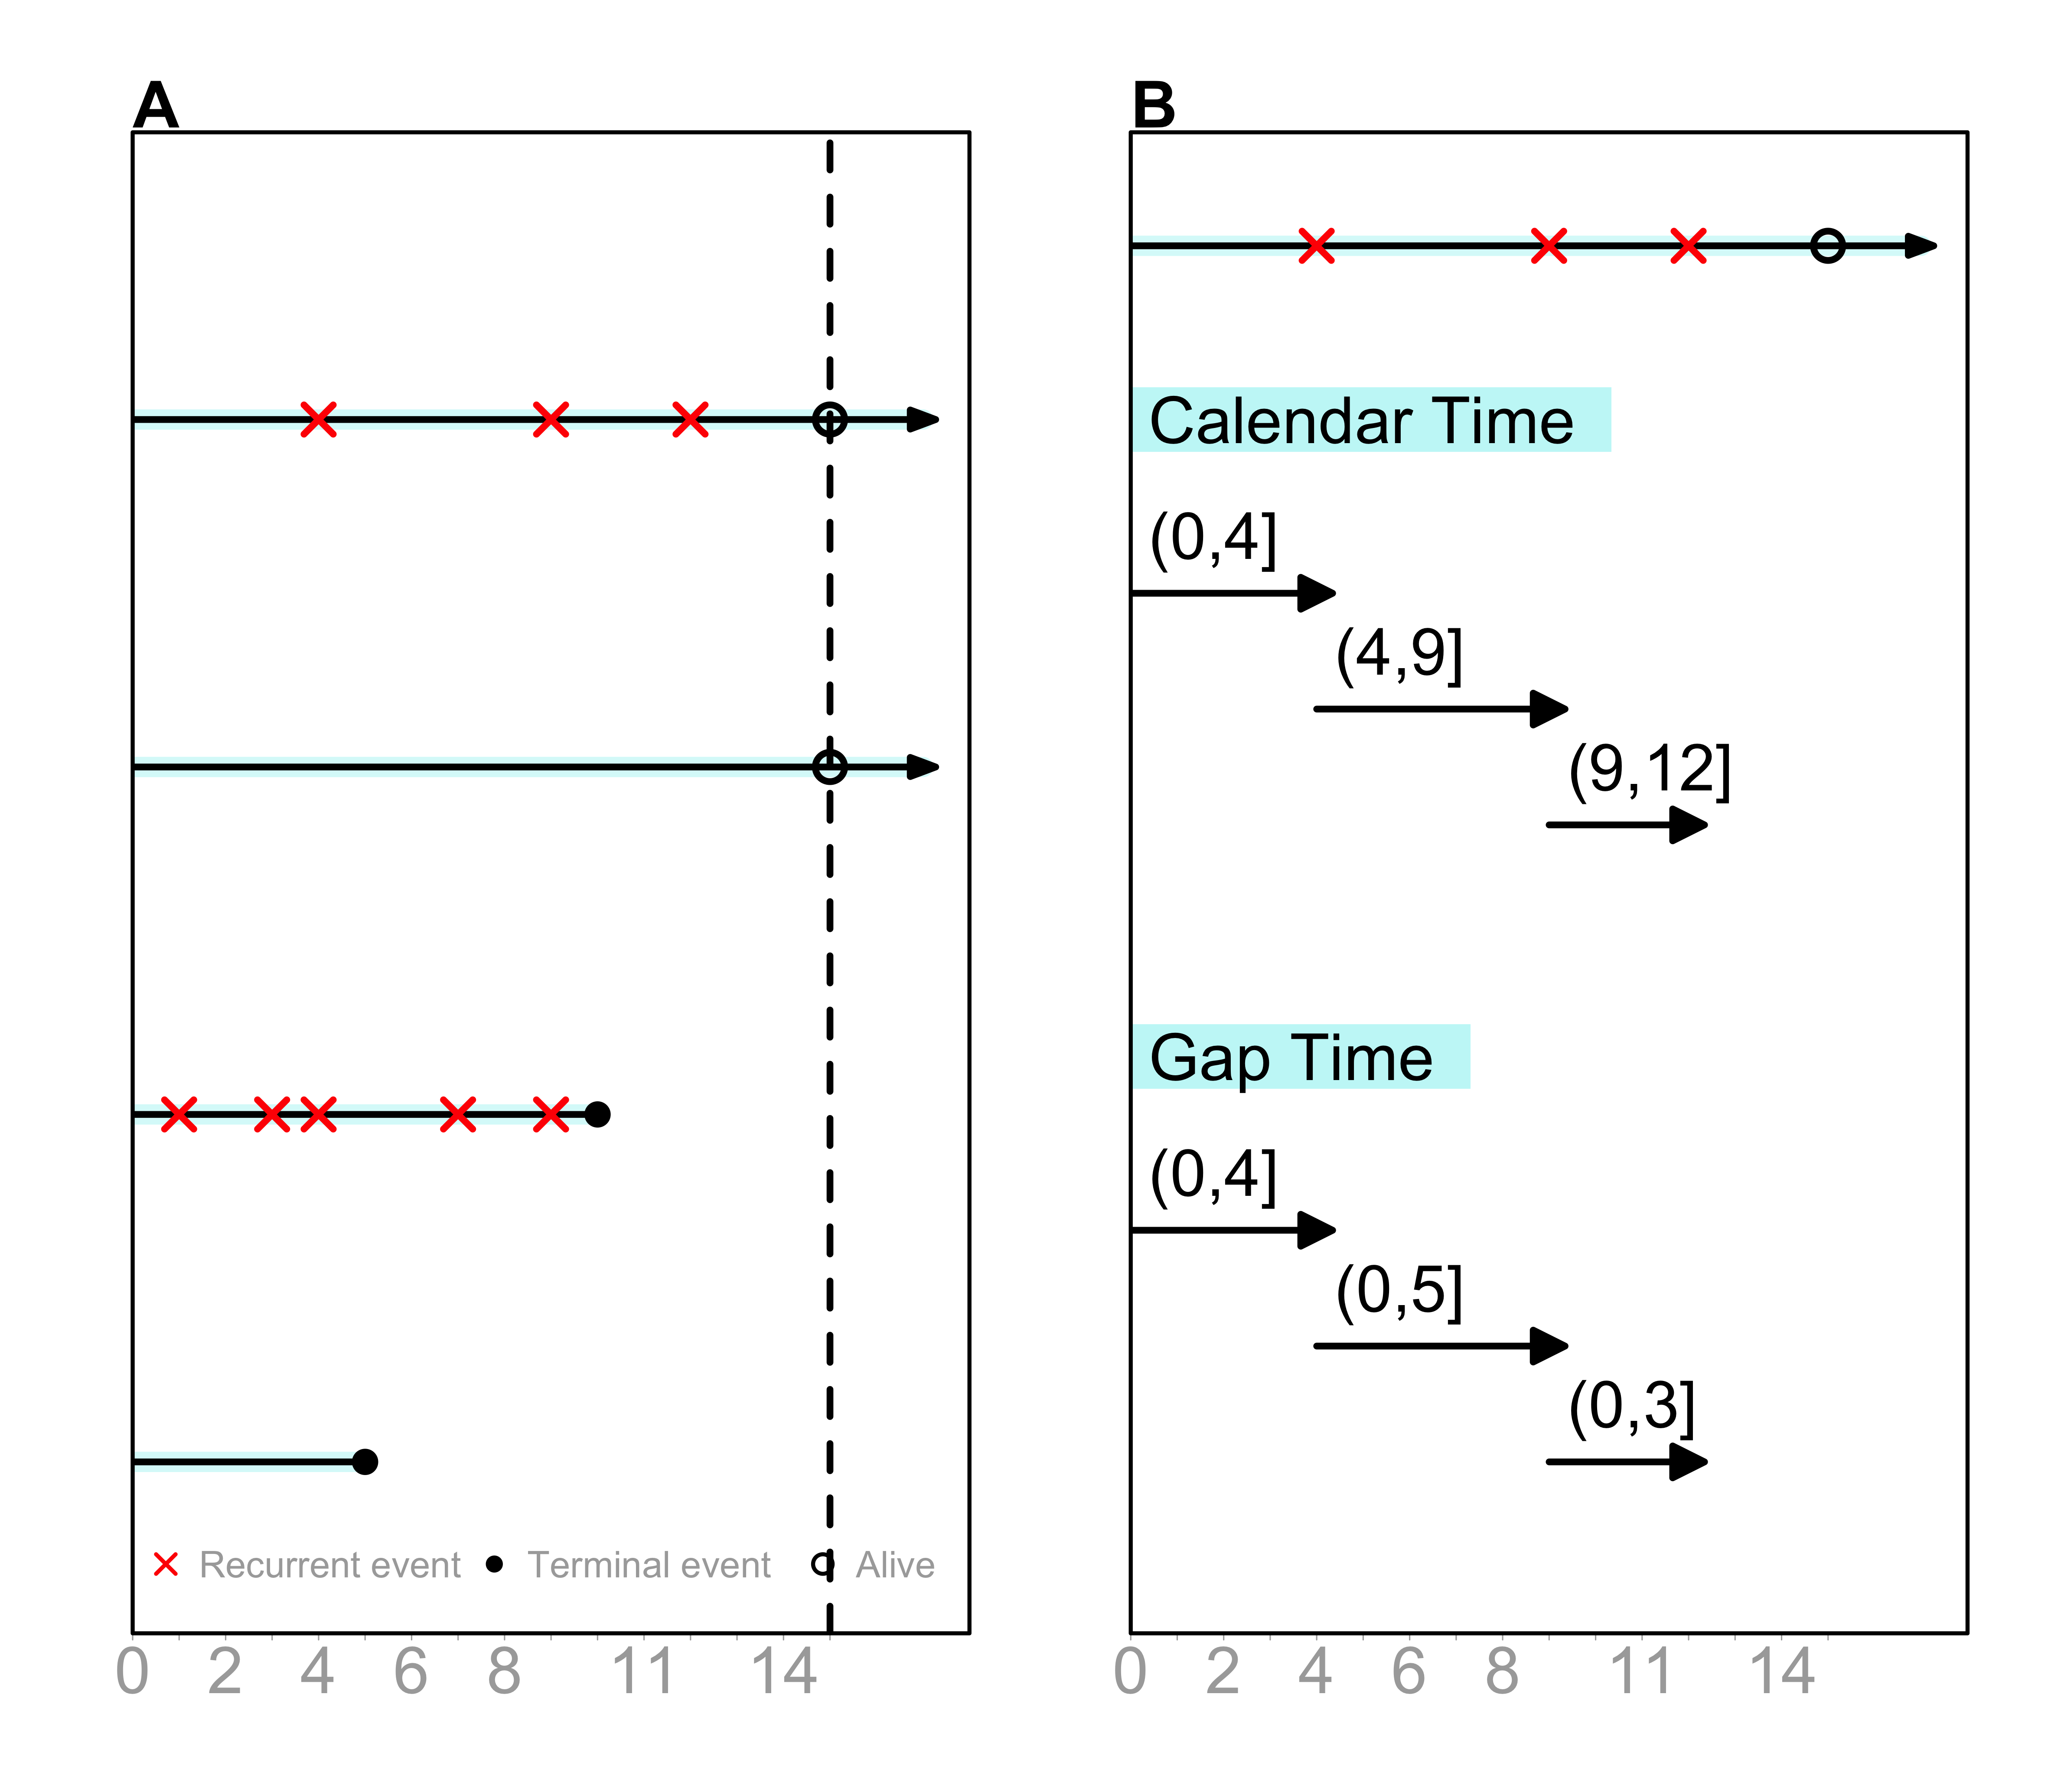
\includegraphics[width=0.9\textwidth]{Figures/Chp3_censor.png}
\caption{Illustrations of data structure and time scales. A: PE occurrences for four selected patients censored at a terminal event or the end of observed period; B: Definitions of risk intervals for calendar time and gap time.}
\label{fig:chp3_censor}
\end{figure}

\section{Joint Model Framework} \label{sec:chp3_mod}

The proposed joint model with shared parameter consists of a longitudinal submodel and an event submodel, specified separately for each type of outcomes. The two submodels are linked using a latent trajectory, which is parameterised in current value and time-dependent slope of the linear predictor. 

\subsection{Longitudinal Submodel}

We define $y_{lij}(t)=y_{li}(t_{lij})$ corresponds to the observed longitudinal outcome for $i^{th}$ ($i=1,\dots,n_l$) individual who comes from $l^{th}$ ($l=1,\dots, L$) center taken at time point $t_{lij}$ ($j=1,\dots,n_{li}$). Then the mixed effects model for $y_{lij}(t)$ takes the form

\begin{align}
&  \left \{\begin{array}{ll}
 y_{lij}(t)=m_{lij}(t)+\epsilon_{lij}(t)\\
 m_{lij}(t)=\bm{x}^T_{lij}(t)\bm{\beta}+b_l+\bm{z}^{T}_{lij}(t)\bm{U}_{li}
\end{array}\right.
\end{align}
where $m_{lij}(t)$ corresponds to the individual linear predictor of observed outcome. $\bm{x}^T_{lij}(t)$ and $\bm{z}^T_{lij}(t)$ are row-vectors of covariates with associated fixed effect coefficient $\bm{\beta}$ and random effects $\bm{U}_{li}$, respectively. The random intercept $b_l$ is set for centers by assuming $b_l \sim N(0,\sigma^2_b)$. The measurement error $\bm{\epsilon}_{li}$ is distributed as $N(\bm{0},\bm{R}_{li})$. As proposed in \cite{Laird1982}, the $\bm{U}_{li}$ are distributed as $N(\bm{0},\bm{D})$, allowing for $\bm{D}$ as an $n_{li} \times n_{li}$ positive-definite covariance matrix, independently of each other and of the $b_l$ and of the $\bm{\epsilon}_{li}$. Further simplification arises when $\bm{R}_{li}=\sigma^2\bm{I}$, where $\bm{I}$ denotes an identity matrix and $\bm{D}=\bm{\Sigma_u}$ with the variance terms ${\sigma^2_{u0}, \sigma^2_{u1}}$ and the correlation coefficient term $\rho$. 

\subsection{Event Submodel}

Let $T_{li}=min(T^{*}_{li},C_{li})$ denote terminal event time where $T^{*}_{li}$ is the so-called 'true' event time and $C_{li}$ is the corresponding censoring time. We define $t_{lik}$ as the observed time for the event submodel with $t_{lik} \leq T_{li}$ $(k \in j)$ and $d_{lik}$ as the event indicator. The individual hazard of a recurrent event using a parametric proportional hazards regression model is given by, 
\begin{align}
    h_{lik}(t)=h_{l0}(t)exp\big\{\bm{\omega}^T_{lik}(t)\bm{\gamma}+f(\bm{\beta},b_l,\bm{U}_{li},\alpha_l;t)+v_{li}\big\}
\end{align}
where $h_{lik}(t)$ denotes $h_{li}(t_{lik})$ for simplicity, $h_{l0}(t)$ is the center-specific baseline hazard, $\bm{\omega}^T_{lik}(t)$ is a row-vector of individual covariates (possibly time-dependent) with corresponding regression coefficient $\bm{\gamma}$ (also known as log hazard ratio). The longitudinal and event processes are assumed to be related via an 'association structure', which is denoted by $f(\cdot)$. In particular, center-specific $\alpha_l$ quantifies the association between the time-varying longitudinal marker and the risk of a recurrent event. Based on our preliminary analysis, we choose current value and current slope of the linear predictor as the association structure, such as

\begin{align}
&  \left \{\begin{array}{ll}
 \mbox{Current value: }f(\bm{\beta}, b_l, \bm{U}_{li}; t)=\alpha_{vl} \times m_{lik}(t)\\
 \mbox{Current slope: }f(\bm{\beta}, b_l, \bm{U}_{li}; t)=\alpha_{sl} \times \frac{d}{dt} m_{lik}(t)
\end{array}\right.
\end{align}
The term $v_{li}$ is a random effect that accounts for the correlation between recurrent events and it is assumed to follow $v_{li} \sim N(0,\sigma^2_v)$  independently. Note that $exp(v_{li})$ is also well known as the frailty term. We further assume that our longitudinal data is non-informative right censoring and the baseline hazard function is modeled with a Weibull distribution, that is $h_{l0}(t)=\delta_l t^{\delta_l-1}$ with $\delta_l$ as center-specific shape parameter. 

\subsection{Assumption}

The key assumption in our proposed joint model is the conditional independence, which means random effects $\bm{b},\bm{U}$ and $\bm{v}$ explain all the interdependence. Let $\bm{\theta}$ denote a vector of all unknown parameters, then we have expressions as followings, 


The longitudinal process is conditionally independent of the event process:
\begin{align}
   p(\bm{t}_{li},\bm{d}_{li},\bm{y}_{li}|b_l,\bm{U}_{li},v_{li};\bm{\theta})=p(\bm{t}_{li},\bm{d}_{li}|b_l,\bm{U}_{li},v_{li};\bm{\theta}) \times p(\bm{y}_{li}|b_l,\bm{U}_{li};\bm{\theta}) 
\end{align}

Recurrent events in the event process are independent of each other: 
\begin{align}
    p(\bm{t}_{li},\bm{d}_{li}|b_l,\bm{U}_{li}, v_{li};\bm{\theta})=\prod_k p(t_{lik},d_{lik}|b_l,\bm{U}_{li},v_{li};\bm{\theta})
\end{align}

Repeated measurements in the longitudinal process are independent of each other: 
\begin{align}
  p(\bm{y}_{li}|b_l,\bm{U}_{li};\bm{\theta})=\prod_j p(y_{lij}|b_l,\bm{U}_{li};\bm{\theta})  
\end{align}

\subsection{Bayesian Inference}

In this section, we specify the posterior distribution, likelihood function of event submodel and prior distributions. All posterior samplings are carried out from the new lightweight R interface \emph{CmdStanr} to \emph{Stan} (\cite{Gelman2013a}, \cite{StanManual}). In both simulation and application study, we obtain 2000 post-warmup posterior samplings via two chains and ensure the convergence by Gelman and Rubin potential scale reduction statistic $\widehat{R}$. Details of elapsed time with system information are included in Appendix \ref{app:c}.  

\subsubsection{Log posterior distribution}

Under the full conditional independence assumption, the individual log posterior distribution can be specified as

\begin{align}
    \begin{split}
        \mbox{log } p(\bm{\theta},b_l,\bm{U}_{li},v_{li}|\bm{y}_{li}, \bm{t}_{li}, \bm{d}_{li}) \propto \mbox{log } & 
        \Big[\prod_jp(y_{lij}|b_l,\bm{U}_{li},\bm{\theta})
        \times \prod_kp(t_{lik},d_{lik}|b_l,\bm{U}_{li},v_{li},\bm{\theta}) \\ & 
        \times p(b_l|\bm{\theta})p(\bm{U}_{li}|\bm{\theta})p(v_{li}|\bm{\theta})p(\bm{\theta})\Big]
    \end{split}
\end{align}

Specifically, the log likelihood function for the event submodel under two scenarios can be rewritten as

\begin{align}
&  \left \{\begin{array}{ll}
 \mbox{Calendar time scale: } \mbox{log } p(t_{lik}, d_{lik}|b_l,\bm{U}_{li},v_{li},\bm{\theta}) = d_{lik} \cdot \mbox{log } h_{li}(t_{lik}) - \int^{t_{lik}}_{t_{li(k-1)}} h_{li}(s)ds \\
 \mbox{Gap time scale: }\mbox{log } p(t_{lik}, d_{lik}|b_l,\bm{U}_{li},v_{li},\bm{\theta}) = d_{lik} \cdot \mbox{log } h_{li}(t_{lik}-t_{li(k-1)}) - \int^{t_{lik}-t_{li(k-1)}}_{0} h_{li}(s)ds
\end{array}\right.
\end{align}
where the latter integral term can be evaluated approximately by Gauss-Kronrod quadrature with Q nodes (\cite{Laurie1997}), such that 

\begin{align}
  \int_a^b h(s)ds \approx \sum^{Q}_{q=1} w_{q,scaled} \cdot h(s_{q,scaled})  
\end{align}
where $w_{q,scaled}=w_q \cdot \frac{b-a}{2}$ and $s_{q,scaled}=\frac{s_q+1}{2}\cdot(b-a)+a$ are scaled weights and locations for quadrature node $q (q=1,\dots, Q)$. The $w_q$ and $s_q$ are standardised wights and locations (also known as abscissa) on interval $[-1,1]$ and we obtain their specific values from the source code of \emph{stan\_jm} from R package \emph{rstanarm} by choosing quadrature nodes $Q=7$.

\subsubsection{Prior distributions}

We identify diffuse or weakly informative but proper priors for all unknown parameters in the proposed joint model. Let $N(\mu,\sigma^2)$ denote normal distribution with location $\mu \in \mathbb{R}$ and scale $\sigma \in \mathbb{R}^{+}$; $t(\nu,\mu,\sigma)$ denote student's t distribution with degrees of freedom $\nu \in \mathbb{R}^{+}$, location $\mu \in \mathbb{R}$ and scale $\sigma \in \mathbb{R}^{+}$; $lkjCorr(\Sigma|\eta) \propto det(\Sigma)^{\eta-1}$ represent LKJ correlation distribution, such that $\Sigma$ is a positive-definite, symmetric matrix with unit diagonal correlation matrix (i.e., a correlation matrix) with shape parameter $\eta \in \mathbb{R}^+$ (see \cite{Lewandowski2009} for details). The prior specifications for the simulation and the application are:

$$\beta_0 \sim N(0,100^2),$$
$$\beta_p \sim N(0,\phi^2_\beta), p=1,2,\dots,P,$$
$$\sigma \sim N(0,\phi^2_\sigma),$$
$$\sigma_b \sim N(0,10^2),$$
$$\sigma_{u0}, \sigma_{u1} \sim t(1,0,10),$$
$$
\begin{bmatrix}
1 & \rho \\
\rho & 1
\end{bmatrix}  \sim lkjCorr(2), $$
$$\gamma_0 \sim N(0,20^2),$$
$$\gamma_q \sim N(0,\phi^2_\gamma), q=1,2,\dots, Q,$$
$$\lambda_l \sim N(0,5^2), l=1,2,\dots,L,$$
$$\sigma_v \sim N(0,10^2)$$
where $\phi_\beta$ and $\phi_\gamma$ are standard deviations of corresponding design matrices and $\phi_\sigma$ is the standard deviation of observed longitudinal outcomes. Practically, \emph{Stan} provides an implicit parameterization of the LKJ correlation matrix density in terms of its Cholesky factor, thus we can set $L_u$ as a Cholesky factor of the correlation matrix $\Sigma=\begin{bmatrix}
1 & \rho \\
\rho & 1
\end{bmatrix}$, such that $L_u \sim \mbox{lkj\_corr\_cholesky}(2)$ implies $\Sigma = L_u \cdot L^{T}_u \sim lkjCorr(2)$. Readers who are interested in this topic can refer to \cite{Sorensen2016} for generating correlated random variables using the Cholesky decomposition. 

\subsection{Individual Prediction}

The individual prediction for the longitudinal marker at time $t$, can be generated from the posterior predictive distribution 
\begin{align} \label{eq:indpred}    
    p(\tilde{y}_{lij}(t)|\mathcal{D})=\int\int\int p(\tilde{y}_{lij}(t)|b_l,\bm{U}_{li},\bm{\theta}) p(b_l,\bm{U}_{li},\bm{\theta}|\mathcal{D}) \,  db_l \,  d\bm{U}_{li} \, d\bm{\theta} 
\end{align}
where $\mathcal{D}=\{\bm{y}_{li},\bm{t}_{li},\bm{d}_{li}; l=1,\dots,L, i=1,\dots,n_l\}$ is the entire collection of data. To compute Equation (\ref{eq:indpred}), we can draw samplings from $p(y_{lij}(t)|b_l^{(m)},\bm{U}_{li}^{(m)},\bm{\theta}^{(m)})$, such that ${b_l^{(m)}, \bm{U}_{li}^{(m)}}$ and $\bm{\theta}^{(m)}$ are the $m^{th}(m=1,\dots,M)$ HMC draws from the joint posterior distribution of $p(b_l,\bm{U}_{li},\bm{\theta}|\mathcal{D})$ as 
\begin{align} \label{eq:indpred2}
  p(\tilde{y}_{lij}(t)|\mathcal{D}) \approx \frac{1}{M} \sum_{m=1}^{M} p(\tilde{y}_{lij}(t)|b_l^{(m)},\bm{U}_{li}^{(m)},\bm{\theta}^{(m)},\mathcal{D}).   
\end{align}
In parallel, for $i^{th}$ individual who has $n^*_{li}(n^*_{li}=0,1,2,\dots)$ recurrent events up to the time $t$, it might be of interest to look beyond and predict the probability of next event-free outcome in the time frame $(t,t']$ with $t'=t+\Delta t$. For this cause, the conditional survival (PE-free) probability can be written as,
\begin{align} \label{eq:cond.surv}
    \begin{split}
        S_{li}(t'|t) & = p(t_{n^*_{li}+1} \geq t'|t_{n^*_{li}+1} > t, \mathcal{D})  \\
                    & = \int\int\int\int p(t_{n^*_{li}+1} \geq t'|t_{n^*_{li}+1} > t, b_l,\bm{U}_{li},v_{li},\bm{\theta},\mathcal{D}) \\
                    & \cdot p(b_l, \bm{U}_{li}, v_{li}, \bm{\theta} |t_{n^*_{li}+1} > t, \mathcal{D}) \, db_l \, d\bm{U}_{li} \, dv_{li} \, d\bm{\theta} \\
        & \approx \frac{1}{M} \sum_{m=1}^{M} exp\Big[ -\int_t^{t'} h\big(s|b_l^{(m)},\bm{U}_{li}^{(m)},v_{li}^{(m)},\bm{\theta}^{(m)}\big) ds \Big]
    \end{split}
\end{align}
where the integration respect to \{$b_l,\bm{U}_{li}, v_{li}, \bm{\theta}$\} is approximated using Monte Carlo method from their posterior samples. The comprehensive derivation of Equation (\ref{eq:cond.surv}) can be found in Appendix \ref{app:c}. The integral term of $\int_{t}^{t'}h(s|\cdot)ds$ can be approximated by Gauss-Kronrod with Q=15 quadrature nodes. The 2.5\% and 97.5\% quantiles of posterior draws from Equation (\ref{eq:cond.surv}) can be obtained as the credible intervals for the predictive probability. 

\subsection{Predictive Performance}

To assess the predictive performance, we employ area under receiver operating characteristic curve (hereafter, AUC) for discrimination (discriminate between individuals who will experience the next recurrent event from subjects who will not) and predictive error for calibration (how well the model predicts the observed event probability). We calculate time-dependent AUC and predictive error under squared loss function based on source code \emph{predictive\_accuracy.stanjm} from R package \emph{rstanarm} and some other nice references (\cite{Andrinopoulou2018}, \cite{Andrinopoulou2021}). The details are described in Table \ref{tab:chp3_auc}.

\begin{table}[H]
\centering \small
\caption{Algorithm for time-dependent AUC and mean predictive error} \label{tab:chp3_auc}
\begin{tabular}{p{14cm}} 
 \toprule
 \textbf{Time-dependent AUC}\\
 \midrule
  \begin{enumerate}
      \item Define individual-specific start time $t_i=\mbox{tstart}_i$ and a common future stop time $t'$. To conform the prediction data, we only include individuals who are still at risk of the event at $t$. For longitudinal data, we adopt observations observed until $t_i$. 
      \item Calculate event-free ('survival') probability at $t'$ and observed $\mbox{tstop}_i$ for each individual based Equation (\ref{eq:cond.surv}) to obtain $S_i(t'|t_i)$ and $S_i(\mbox{tstop}_i|t_i)$
      \item Sort individuals by their observed $\mbox{tstop}$ in an increasing order and group each two by combinations without replacement. 
      \item AUC is calculated by accounting for weights caused by censoring conditions. For each combation $c=1,\dots,C$, assume that $\mbox{tstop}_i < \mbox{tstop}_j$:
        \begin{itemize}
            \footnotesize
            \item If only individual $i$ is censored at $t'$, which means $\mbox{tstop}_i \leq t'$ \& $\mbox{status}_i=0$, then weight $w=1-S_i(\mbox{tstop}_i|t_i)$
            \item If only individual $j$ is censored at $t'$, which means $\mbox{tstop}_j \leq t'$ \& $\mbox{status}_j=0$, then weight $w=S_j(\mbox{tstop}_j|t_j)$
            \item If both individuals are censored at $t'$, then weight $w=\big(1-S_i(\mbox{tstop}_i|t_i)\big) \times S_j(\mbox{tstop}_j|t_j)$
            \item If it does not belong to above cases, $w=1$
            \item Let $S_i=S_i(t'|t_i), S_j=S_j(t'|t_j)$, compute $A_c=I_{S_i<S_j} \cdot w$; $D_c=I_{S_i>S_j} \cdot w$; $T_c=I_{S_i=S_j} \cdot w$, where $I_x$ denotes a indicator function with 1 when $x$ is true and 0, otherwise. 
        \end{itemize}
      \item Repeat Step 4 until $C$ times
      \item $\mbox{AUC}=\sum_{c=1}^C \big(\frac{A_c+0.5 \cdot T_c}{A_c + D_c + T_c}\big)$
   \end{enumerate}\\
    \hline
 \textbf{Time-dependent mean predictive error (MPE)}\\
 \midrule
 \begin{enumerate}
     \item  For each individual $i (i=1,\dots,N)$: 
         \begin{itemize}
         \footnotesize
             \item If individual $i$ died or censored after $t'$, $\mbox{Error}_i=(1-S_i)^2$
             \item If individual $i$ died before $t'$, $\mbox{Error}_i=(0-S_i)^2$
             \item If individual $i$ censored before $t'$, $\mbox{Error}_i=S_i(\mbox{tstop}_i|t_i) \times (1-S_i)^2+\big(1-S_i(\mbox{tstop}_i|t_i)\big) \times (0-S_i)^2$
         \end{itemize}
    \item Mean Predictive Error (MPE)=$\frac{\sum_{i=1}^{N}\mbox{Error}_i}{N}$
 \end{enumerate}\\
 \bottomrule
 \hline
\end{tabular}
\end{table}

\subsection{Model Selection}

We allude to the leave-one-out (LOO) cross-validation for model choice, which in its own words is the method for estimating pointwise out-of-sample prediction accuracy from the log-likelihood evaluated at the posterior simulations of the parameter values. \cite{Vehtari2017} developed an efficient computation for LOO using Pareto-smoothed importance sampling (PSIS) to lay out fast and stable computations for LOO. PSIS-LOO is demonstrated to be even more robust than asymptotic widely applicable information criterion (WAIC) (\cite{Watanabe2010}), which is a recent popular measure of predictive accuracy. We implement the computations of LOO information criterion (LOOIC) via R package \emph{loo} (v2.3.1, \cite{Vehtari2020}) by extracting log likelihoods from posterior samplings.  

The PSIS estimate of expected log pointwise predictive density (elpd) is 
\begin{align} \label{eq:loo}
    \widehat{\mbox{elpd}}_{\mbox{psis-loo}}=\sum_{l=1}^{L}\sum_{i=1}^{n_l}log\Big(\frac{\sum_{s=1}^S w^s_{li}p(y_{li}|\theta^s)}{\sum_{s=1}^S w^s_{li}} \Big)
\end{align}
 where $w^s_{li}$ denotes weights at iteration $s$, $p(y_{li}|\theta^s)$ denotes likelihood function at $s$. As with WAIC, we define LOOIC as $-2$ times the Equation (\ref{eq:loo}) so as to be on the deviance scale. Analogously, the model with smaller LOOIC value indicates the better goodness of fit. 
 
\section{Simulation} \label{sec:chp3_sim}

We simulate a total of four hierarchical data sets and fit to corresponding proposed joint models, with the aim to assess the performance of each proposed joint model in a comparison of the two-stage approach. Four proposed joint models are summarized as: i) joint model with current slope as the association structure and gap time as the time scale (hereafter, Slope+Gap); ii) joint model with current slope as the association structure and calendar time as the time scale (hereafter, Slope+Calendar); iii) joint model with current value as the association structure and gap time as the time scale (hereafter, Value+Gap); iv) joint model with current value as the association structure and calendar time as the time scale (hereafter, Value+Calendar). 

\begin{table}[H]
\small\centering
\caption{Simulation progress} \label{tab:chp3_sim}
\begin{tabular}{p{14cm}} 
 \toprule
 {\normalsize \bf Simulation algorithm} \\
 \midrule
  \textbf{\emph{Random effects}}\\
     Simulate $b_l \sim N(0,\sigma_b^2)$, $\bm{U_i}=(U_{0i},U_{1i})^T \sim N(\bm{0},\bm{\Sigma}_u)$, and $\bm{\Sigma}_u$ is the covariance matrix with the variance terms $\sigma^2_{u0}, \sigma^2_{u1}$ and the correlation coefficient term $\rho$ \\
   \midrule 
   
   \bf Event Process
    \hspace{0.5cm} \
    \begin{enumerate}
        \item \textbf{\emph{Terminal event}} 
            \begin{itemize}
                \item Simulate $\omega_1 \sim \mbox{Bernoulli}(0.5), \omega_2 \sim N(0,1), v_i \sim N(0,\sigma^2_v), u_i \sim \mbox{Uniform}(0,1)$
                \item Let $A=\gamma_0+\gamma_1\omega_1+\gamma_2\omega_2$
                \item Define hazard function with Weibull as the baseline hazard, that is $h_{i}(t)=\delta_l t ^{\delta_l-1} exp(A)$
                \item Cumulative hazard function $H_i(t)=\int_{0}^{t}h_{i}(s)ds$
                \item Solve $t$ from equation $H_i(t)+log(u_i)=0$
                \item Terminal time $T_i=min(t,t_{\mbox{max}})$, where maximum follow-up time $t_{\mbox{max}}=10$ years
            \end{itemize}
        \item \textbf{\emph{Recurrent event}}
            \begin{itemize}
                 \item Let $f(\beta,b_l,\bm{U}_i;t)=\alpha_{vl} \cdot m_{ik}(t)/\alpha_{sl} \cdot m'_{ik}(t)$, where $m_{ik}(t)=\beta_0+\beta_1 t+\beta_2 t^2+b_l+U_{0i}+U_{01} \cdot t$
                \item Hazard function of $k^{th}$ event: $h_{ik}(t)=\delta_l t ^{\delta_l-1} exp(A+ f(\beta,b_l,\bm{U}_i;t) + v_i)$
                \item Set starting point: $\mbox{tstart}_{i0}=0$
                \item In each loop $k=1,\dots,K$, generate $u_{ik}\sim \mbox{Uniform}(0,1)$
                \item If time scale is set as gap: Solve $\Delta t_{ik}$ from equation $H_i(\Delta t_{ik})+log(u_{ik})=0$, where $H_i(\Delta t_{ik})=\int_{0}^{\Delta t_{ik}}h_{ik}(s)ds=$
               $\int_{0}^{\Delta t_{ik}}\delta_l s^{\delta_l-1}exp\big(A+f(\beta,b_l,\bm{U}_i;s+\mbox{tstart}_{ik})+v_i\big)ds$
                \item If time scale is set as calendar: Solve $\Delta t_{ik}$ from equation $H_i(\Delta t_{ik})+log(u_{ik})=0$, where $H_i(\Delta t_{ik})=\int_{0}^{\Delta t_{ik}}h_{ik}(s)ds=$ 
               $\int_{0}^{\Delta t_{ik}}\delta_l (s+\mbox{tstart}_{ik})^{\delta_l-1}exp\big(A+f(\beta,b_l,\bm{U}_i;s+\mbox{tstart}_{ik})+v_i\big)ds$
             \item Update $\mbox{tstart}_{ik}=\mbox{tstart}_{i(k-1)}+\Delta t_{ik}+ \mbox{28 days}$, $\mbox{tstop}_{i(k-1)}=\mbox{tstart}_{i(k-1)}+\Delta t_{ik}$ until $\mbox{tstart}_{ik}$ reaches up to $T_i$
            \end{itemize}
    \end{enumerate}\\
      \midrule 
   \textbf{Longitudinal Process}\\ 
   %\hspace{0.5cm} \textbf{\emph{Longitudinal marker}}: \\
    Once $\mbox{tstop}_{i(k-1)}$ is obtained from the previous step, we adjust $t_{ij}=\mbox{tstop}_{i(k-1)}$ for $j=2,\dots,K+1$ and set $t_{ij}=0$ for $j=1$, such that $y_{ij}=m_{ij}(t_{ij})+\epsilon_{ij}$,
  where $\epsilon_{ij} \sim N(0,\sigma^2)$\\
      \bottomrule
\end{tabular}
\end{table}

We simulate each data set consisting of an average of 480 individuals who are from $L=6$ centers for 50 replicates for each proposed joint model. The data generating algorithm is shown in Table \ref{tab:chp3_sim}. It is worth noting that we add a fixed time window (28 days) to mimic the real case by accounting for patients' recovery time. Comparisons between estimate and true value of each parameter are displayed in Figure \ref{fig:chp3_est1} and Figure \ref{fig:chp3_est2}. We observe that both joint model and two-stage approaches yield to reasonable fitting performance. Nonetheless, there exists the need to investigate both approaches in a real data example, which will be discussed in the next section. Details for explicit true values, estimates are described in Appendix \ref{app:c}.  

\begin{figure}[ht] 
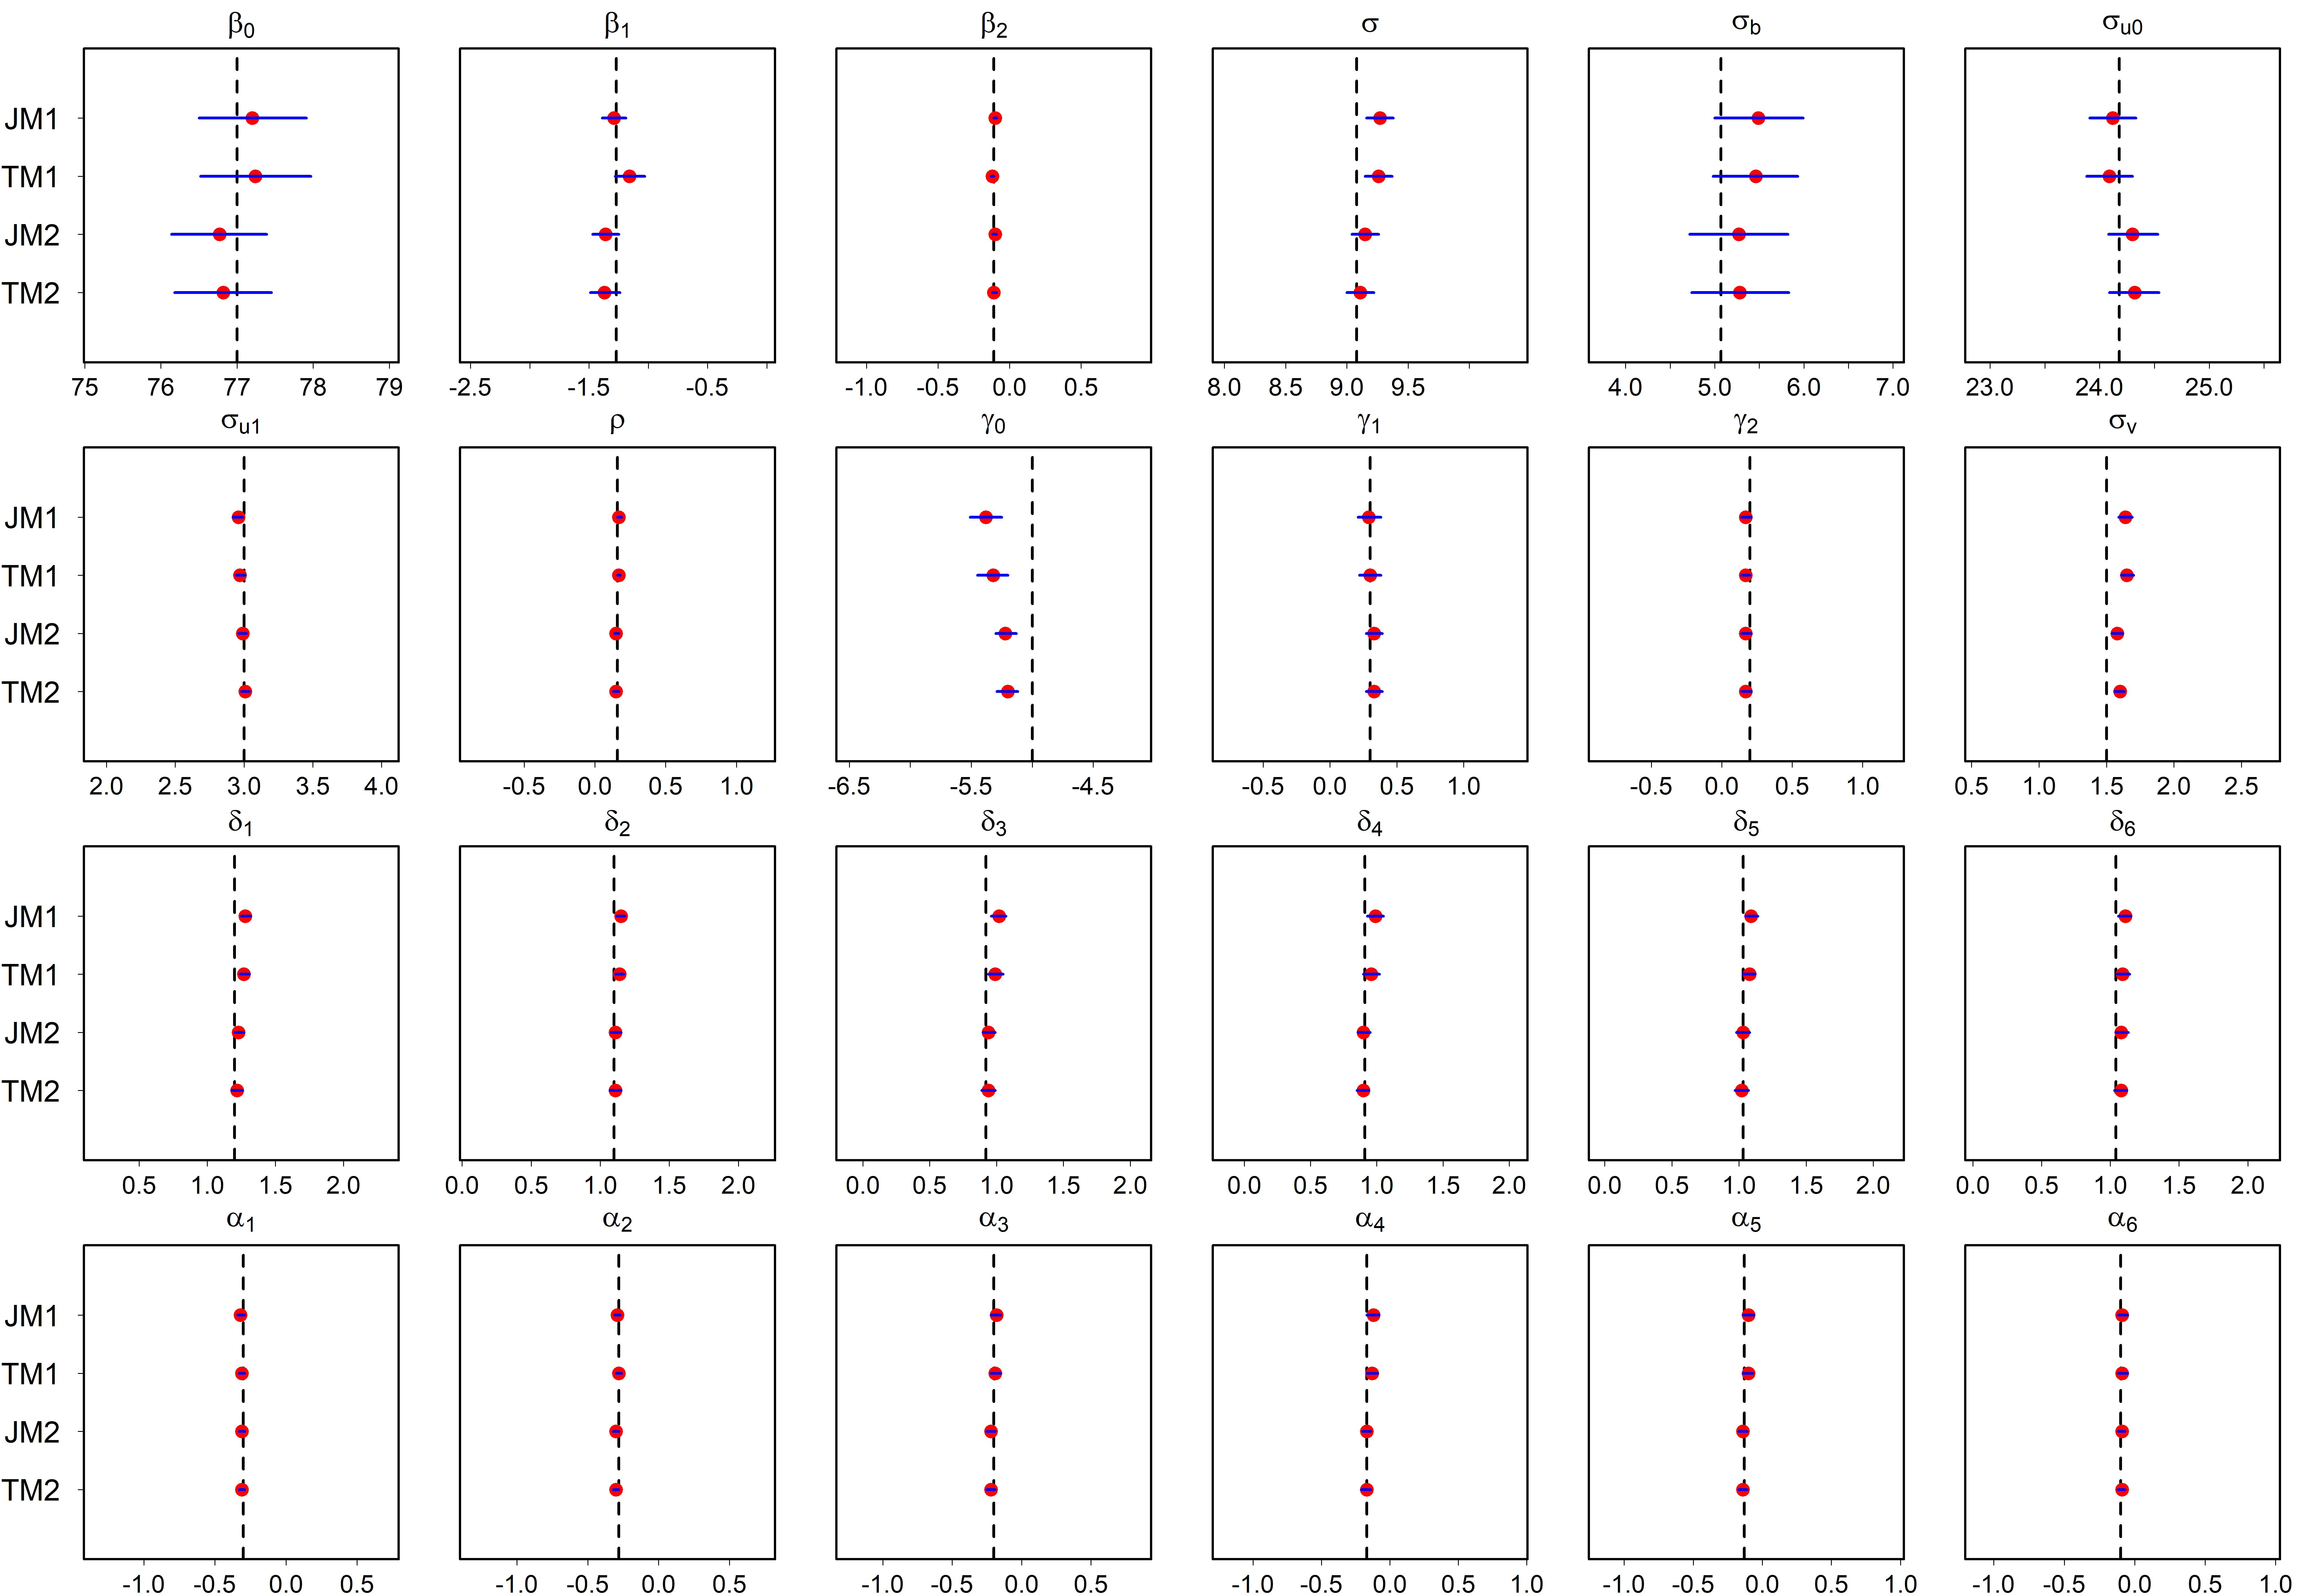
\includegraphics[width=\textwidth]{Figures/Chp3_sim_1.jpg} 
\caption{Simulation results based on 50 replicates with true value (dashed vertical line), posterior mean estimates (red dot) and corresponding 95\% confidence interval (blue line). JM1: Joint model Slope+Gap; TM1: Two-stage model Slope+Gap; JM2: Joint model Slope+Calendar; TM2: Two-stage model Slope+Calendar}
\label{fig:chp3_est1}
\end{figure}

\begin{figure}[ht] 
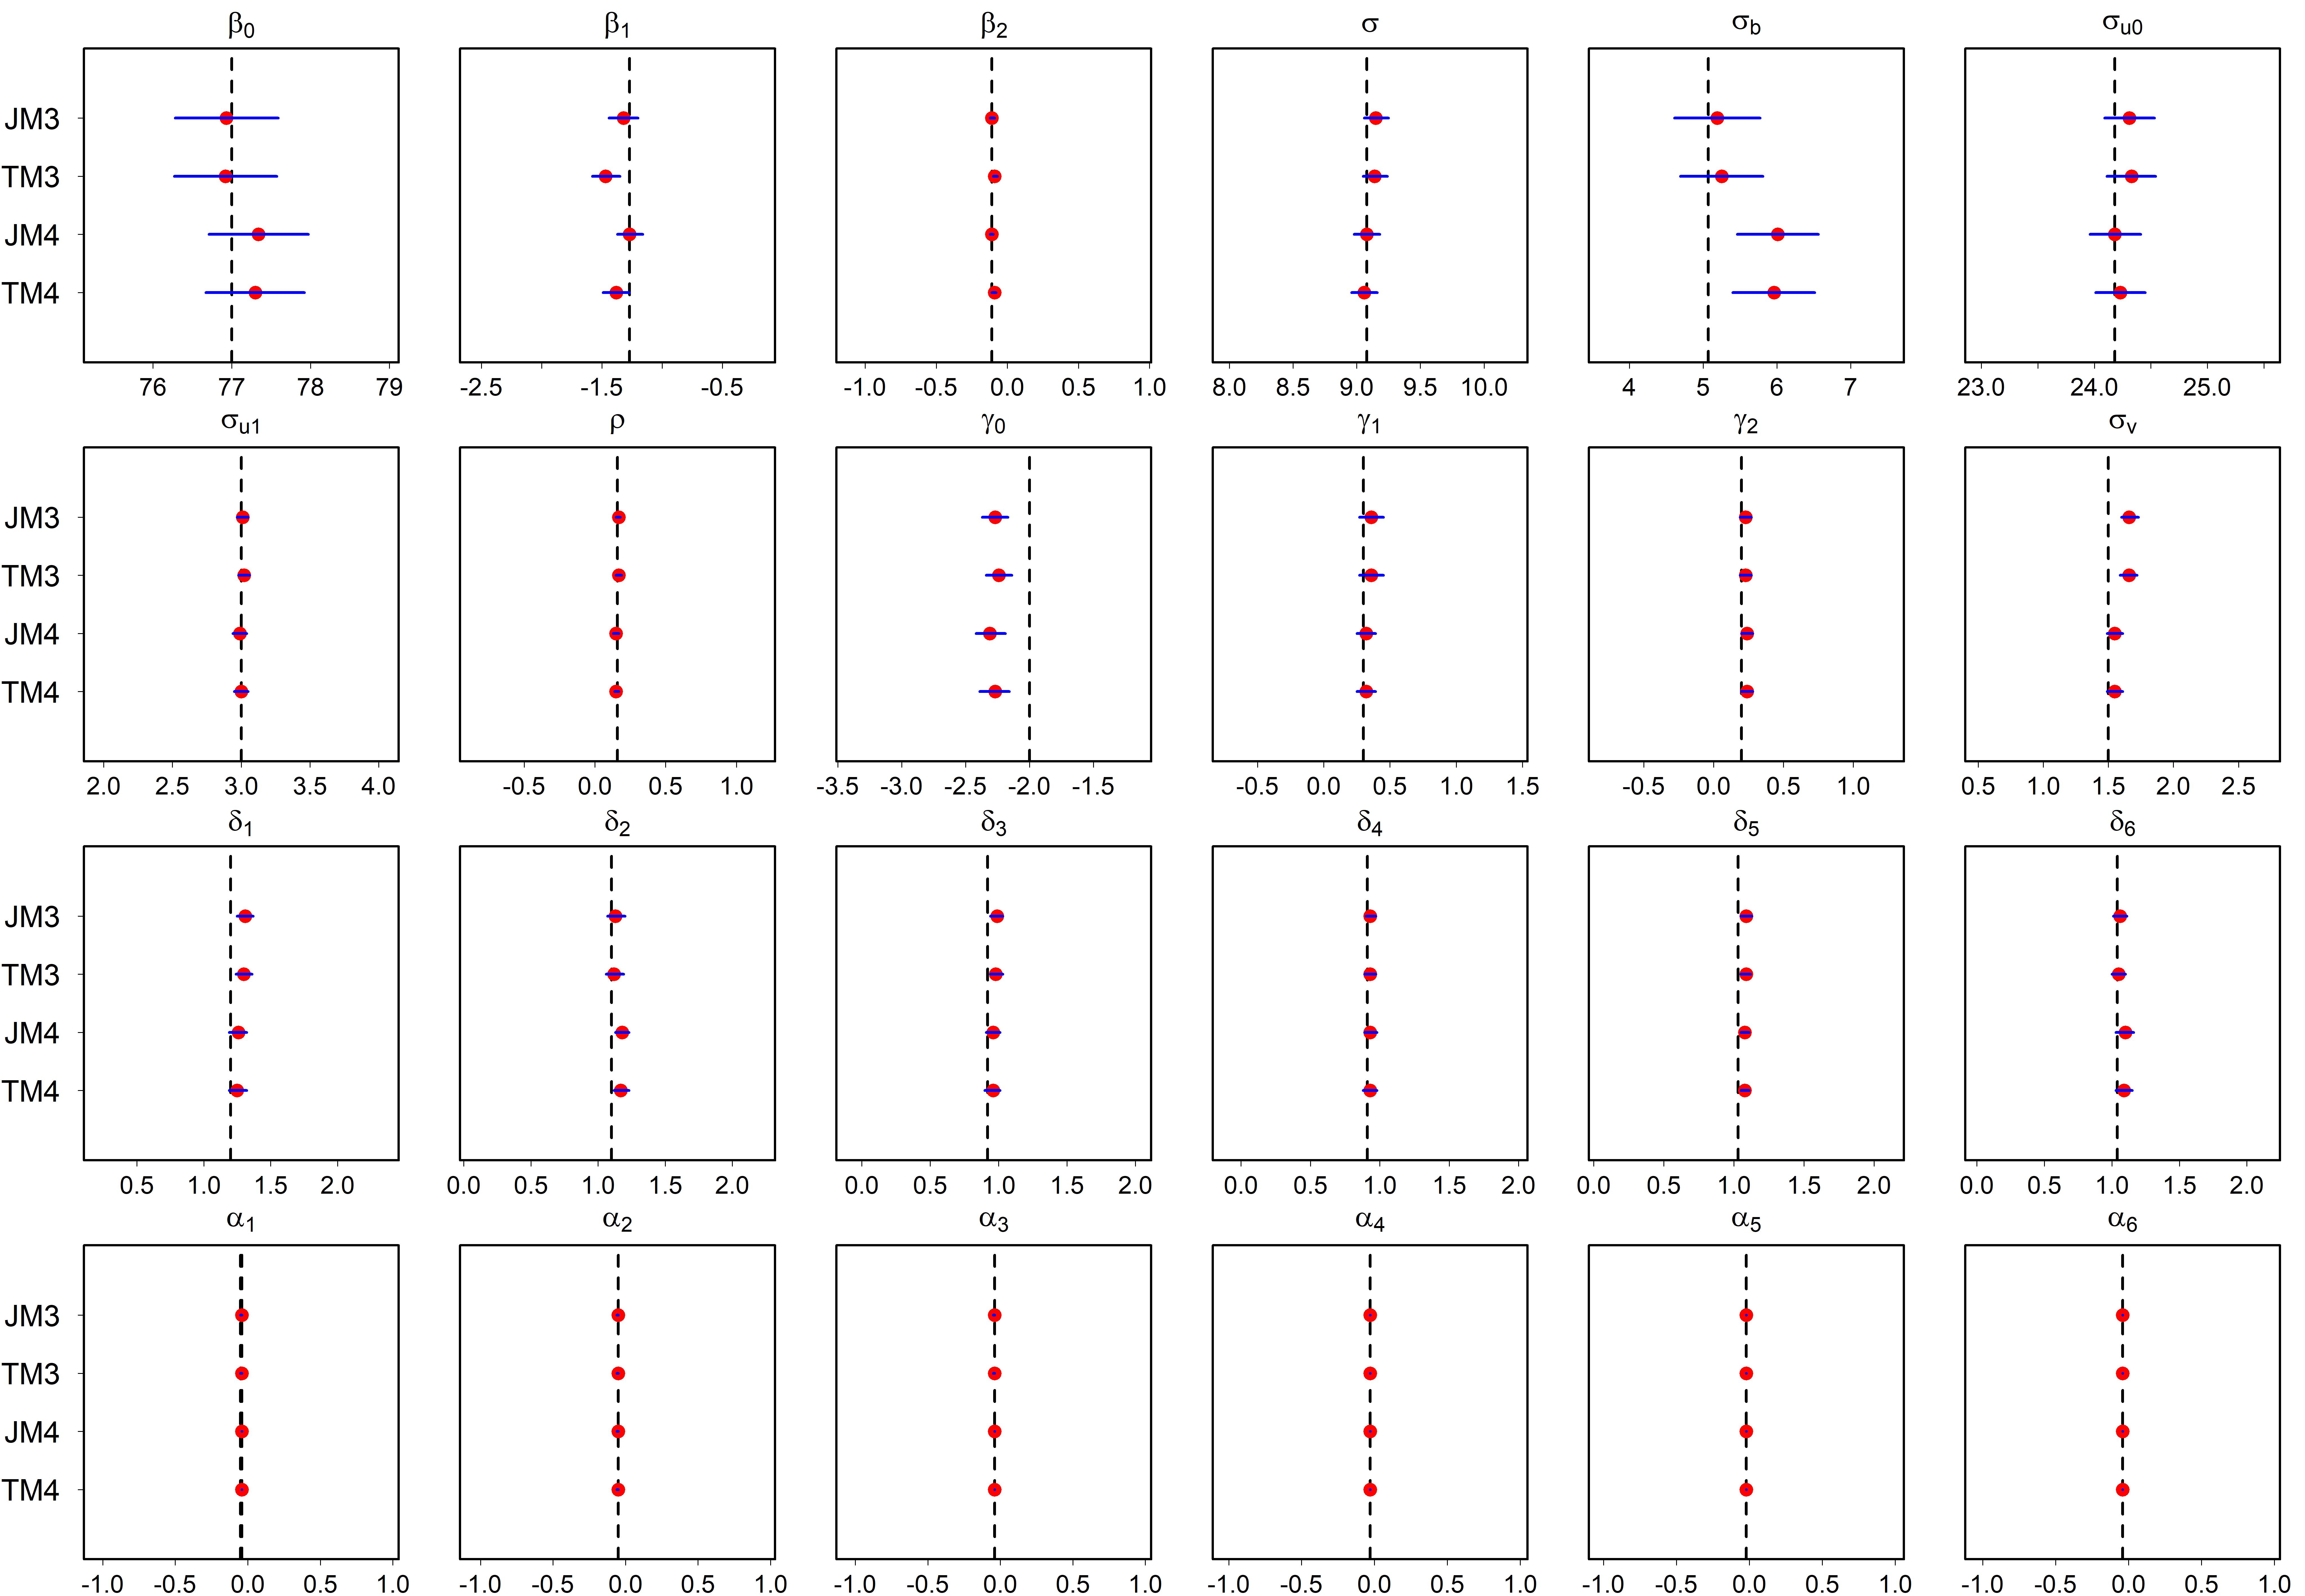
\includegraphics[width=\textwidth]{Figures/Chp3_sim_2.jpg}
\caption{Simulation results based on 50 replicates with true value (dashed vertical line), posterior mean estimates (red dot) and corresponding 95\% confidence interval (blue line). JM3: Joint model Value+Gap; TM3: Two-stage model Value+Gap; JM4: Joint model Value+Calendar; TM4: Two-stage model Value+Calendar}
\label{fig:chp3_est2}
\end{figure}

\section{Application} \label{sec:chp3_app}

In this section, we illustrate our motivating multi-center CF study, which tracked the lung trajectory and corresponding covariates of patients since 1997 by US CF Foundation Registry. Our study was approved by the Institutional Review Boards at Cincinnati Children’s Hospital Medical Center and University of Cincinnati.

The details of data cleaning process are described in Appendix \ref{app:c}. The final cleaned data we obtained is of 440 patients, which 178 (40.45\%) patients never encounter PE, 7 (1.59\%) patients experience PE only once, 255 (57.95\%) patients experience recurrent events during the follow-up period. Descriptive statistics by centers are summarized in Table \ref{tab:chp3_dem}, of which includes: i) demographic summary, such as Gender, Genotype, Birth cohort; ii) the first recorded covariates, such as baseline age and baseline ppFEV1; iii) binary time-varying measures on insurance use, microbiology (infection with pa or MRSA) and \emph{CF-related diabetes mellitus} (cfrd). The time since baseline is utilized as the time scale for analysis. The category levels of birth cohort are computed by quartile 0-25\%, 25\%-50\%, 50\%-75\% and 75\%-100\%, respectively. This covariate may offer some remedies for biases induced by left-truncation from review year 2003. To account for irregular visit due to disease severity, we have included numbers of PEs and outpatient visits within the year prior to a given clinical encounter as predictors. Trajectory in Figure \ref{fig:chp3_traj} displays the heterogeneous nature of lung function and recurrent feature of PE over the life span. We note that PE events are more likely to appear when the averaged values of ppFEV1 are low.   

\begin{table}[H]
  \footnotesize\sf\centering
  \captionsetup{justification=centering}
   \caption{Demographic clinical summary across centers} \label{tab:chp3_dem}
    \begin{threeparttable}
 \begin{tabular}{lcccccc}
    \toprule
  & \textbf{\specialcell{Center 1\\(N=74)}} & \textbf{\specialcell{Center 2\\(N=70)}} & \textbf{\specialcell{Center 3\\(N=75)}} & \textbf{\specialcell{Center 4\\(N=75)}} & \textbf{\specialcell{Center 5\\(N=72)}} & \textbf{\specialcell{Center 6\\(N=74)}} \\
 \midrule
\rowcolor{Gainsboro!60}
 \multicolumn{7}{l}{\textbf{Baseline age (years)}} \\[2pt]
 \hspace{0.5cm} \specialcell{Mean; Median\\(Min - Max)} &  \specialcell{19.0; 17.0\\(6.08 - 47.6)} & \specialcell{29.4; 21.9\\ (17.7 - 79.8)} & \specialcell{15.7; 13.5\\ (6.11 - 63.9)} & \specialcell{17.7; 14.7\\ (6.04 - 53.4)} & \specialcell{11.3; 10.6\\ (6.02 - 34.6)} &	\specialcell{17.4; 15.0\\ (6.01 - 51.9)}\\
\rowcolor{Gainsboro!60}
 \multicolumn{7}{l}{\textbf{Baseline ppFEV1}} \\[2pt]
 \hspace{0.5cm} \specialcell{Mean; Median\\(Min - Max)} & \specialcell{77.4; 79.2\\ (16.2 - 144)} & \specialcell{64.7; 65.8\\ (25.3 - 111)} & \specialcell{80.5; 83.5\\ (23.7 - 134)}	& \specialcell{82.2; 88.7\\ (19.7 - 117)}	& \specialcell{80.4; 85.8\\ (18.3 - 129)} & \specialcell{79.6; 80.4 \\ (19.6 - 129)}\\
 \rowcolor{Gainsboro!60}
 \multicolumn{7}{l}{\textbf{Gender}} \\[2pt]
 \hspace{0.5cm} Female & 23 (31.1\%) & 31 (44.3\%) & 31 (41.3\%) & 30 (40.0\%) & 24 (33.3\%) & 25 (33.8\%)\\ 
 \hspace{0.5cm} Male & 51 (68.9\%) & 39 (55.7\%) & 44 (58.7\%) & 45 (60.0\%) & 48 (66.7\%) & 49 (66.2\%)\\
 \rowcolor{Gainsboro!60}
 \multicolumn{7}{l}{\textbf{Genotype (F508del)}} \\[2pt]
 \hspace{0.5cm} Neither/Unknown & 30 (40.5\%) &	14 (20.0\%) & 10 (13.3\%) &	17 (22.7\%) & 14 (19.4\%) & 13 (17.6\%)\\
 \hspace{0.5cm} Homozygous & 11 (14.9\%) & 22 (31.4\%) & 40 (53.3\%) & 28 (37.3\%) & 30 (41.7\%) &	28 (37.8\%)\\
 \hspace{0.5cm} Heterozygous & 33 (44.6\%) & 34 (48.6\%) & 25 (33.3\%) & 30 (40.0\%) & 28 (38.9\%) & 33 (44.6\%)\\
 \rowcolor{Gainsboro!60}
  \multicolumn{7}{l}{ \textbf{Birth cohort}} \\[2pt]
 \hspace{0.5cm} $<1988$ & 16 (21.6\%) &	26 (37.1\%) & 20 (26.7\%) &	28 (37.3\%) & 5 (6.9\%) & 30 (40.5\%)\\
 \hspace{0.5cm} $[1988,1993)$ & 14 (18.9\%) & 21 (30.0\%) &	13 (17.3\%) &	19 (25.3\%) & 20 (27.8\%) & 13 (17.6\%)\\
 \hspace{0.5cm} $[1993,1998)$ & 12 (16.2\%) & 23 (32.9\%) &	13 (17.3\%) &	11 (14.7\%) & 19 (26.4\%) & 16 (21.6\%)\\
 \hspace{0.5cm} $>1998$ & 32 (43.2\%) &	0 (0\%)	& 29 (38.7\%) &	17 (22.7\%)&	28 (38.9\%) & 15 (20.3\%)\\
 \rowcolor{Gainsboro!60}
 \multicolumn{7}{l}{\textbf{Insurance use}} \\[2pt]
 \hspace{0.5cm} At baseline & 44 (59.5\%) & 8 (11.4\%) & 49 (65.3\%) &	58 (77.3\%) & 33 (45.8\%) & 37 (50.0\%)\\
 \hspace{0.5cm} Ever during follow-up & 53 (71.6\%) & 17 (24.3\%) & 70 (93.3\%) &	68 (90.7\%) & 48 (66.7\%) &	50 (67.6\%)\\
 \rowcolor{Gainsboro!60}
 \multicolumn{7}{l}{\textbf{Pseudomonas aeruginosa (pa)}} \\[2pt]
 \hspace{0.5cm} Baseline & 19 (25.7\%) & 15 (21.4\%) & 18 (24.0\%) & 22 (29.3\%) & 15 (20.8\%) & 17 (23.0\%)\\
 \hspace{0.5cm} Ever follow-up & 36 (48.6\%) & 41 (58.6\%) & 49 (65.3\%) & 47 (62.7\%) & 54 (75.0\%) & 47 (63.5\%)\\
 \rowcolor{Gainsboro!60}
 \multicolumn{7}{l}{\textbf{Methicillin-resistant Staphylococcus aureus (MRSA)}} \\[2pt]
 \hspace{0.5cm} At baseline & 18 (24.3\%) & 2 (2.9\%) & 11 (14.7\%) & 5 (6.7\%) & 7 (9.7\%) & 3 (4.1\%)	\\
 \hspace{0.5cm} Ever during follow-up & 28 (37.8\%) & 19 (27.1\%) & 41 (54.7\%) & 21 (28.0\%) &	37 (51.4\%) & 30 (40.5\%) \\
 \rowcolor{Gainsboro!60}
  \multicolumn{7}{l}{\textbf{CF-related diabetes mellitus (cfrd)}} \\[2pt]
 \hspace{0.5cm} At baseline & 9 (12.2\%) &	16 (22.9\%) & 6 (8.0\%) & 8 (10.7\%) & 7 (9.7\%) & 7 (9.5\%)\\
 \hspace{0.5cm} Ever during follow-up & 22 (29.7\%) & 24 (34.3\%) & 32 (42.7\%) &	33 (44.0\%) & 23 (31.9\%) & 33 (44.6\%)\\
 \rowcolor{Gainsboro!60}
  \multicolumn{7}{l}{\textbf{On Enzymes}}\\[2pt]
 \hspace{0.5cm} At baseline & 53 (71.6\%) & 58 (82.9\%) & 38 (50.7\%) & 27 (36.0\%) & 30 (41.7\%) & 25 (33.8\%)\\
 \hspace{0.5cm} Ever during follow-up & 60 (81.1\%) & 61 (87.1\%) & 68 (90.7\%) &	69 (92.0\%) & 71 (98.6\%) &	63 (85.1\%)\\
 \rowcolor{Gainsboro!60}
  \multicolumn{7}{l}{\textbf{PE event}}\\[2pt]
 \hspace{0.5cm} At baseline & 22 (29.7\%) & 25 (35.7\%) & 14 (18.7\%) & 17 (22.7\%) & 29 (40.3\%) & 17 (23.0\%)\\
 \hspace{0.5cm} Ever during follow-up & 49 (66.2\%) & 30 (42.9\%) & 42 (56.0\%) &	42 (56.0\%) & 58 (80.6\%) & 39 (52.7\%)\\
    \bottomrule
  \end{tabular}
    \end{threeparttable}
\end {table}

\begin{figure}[ht]
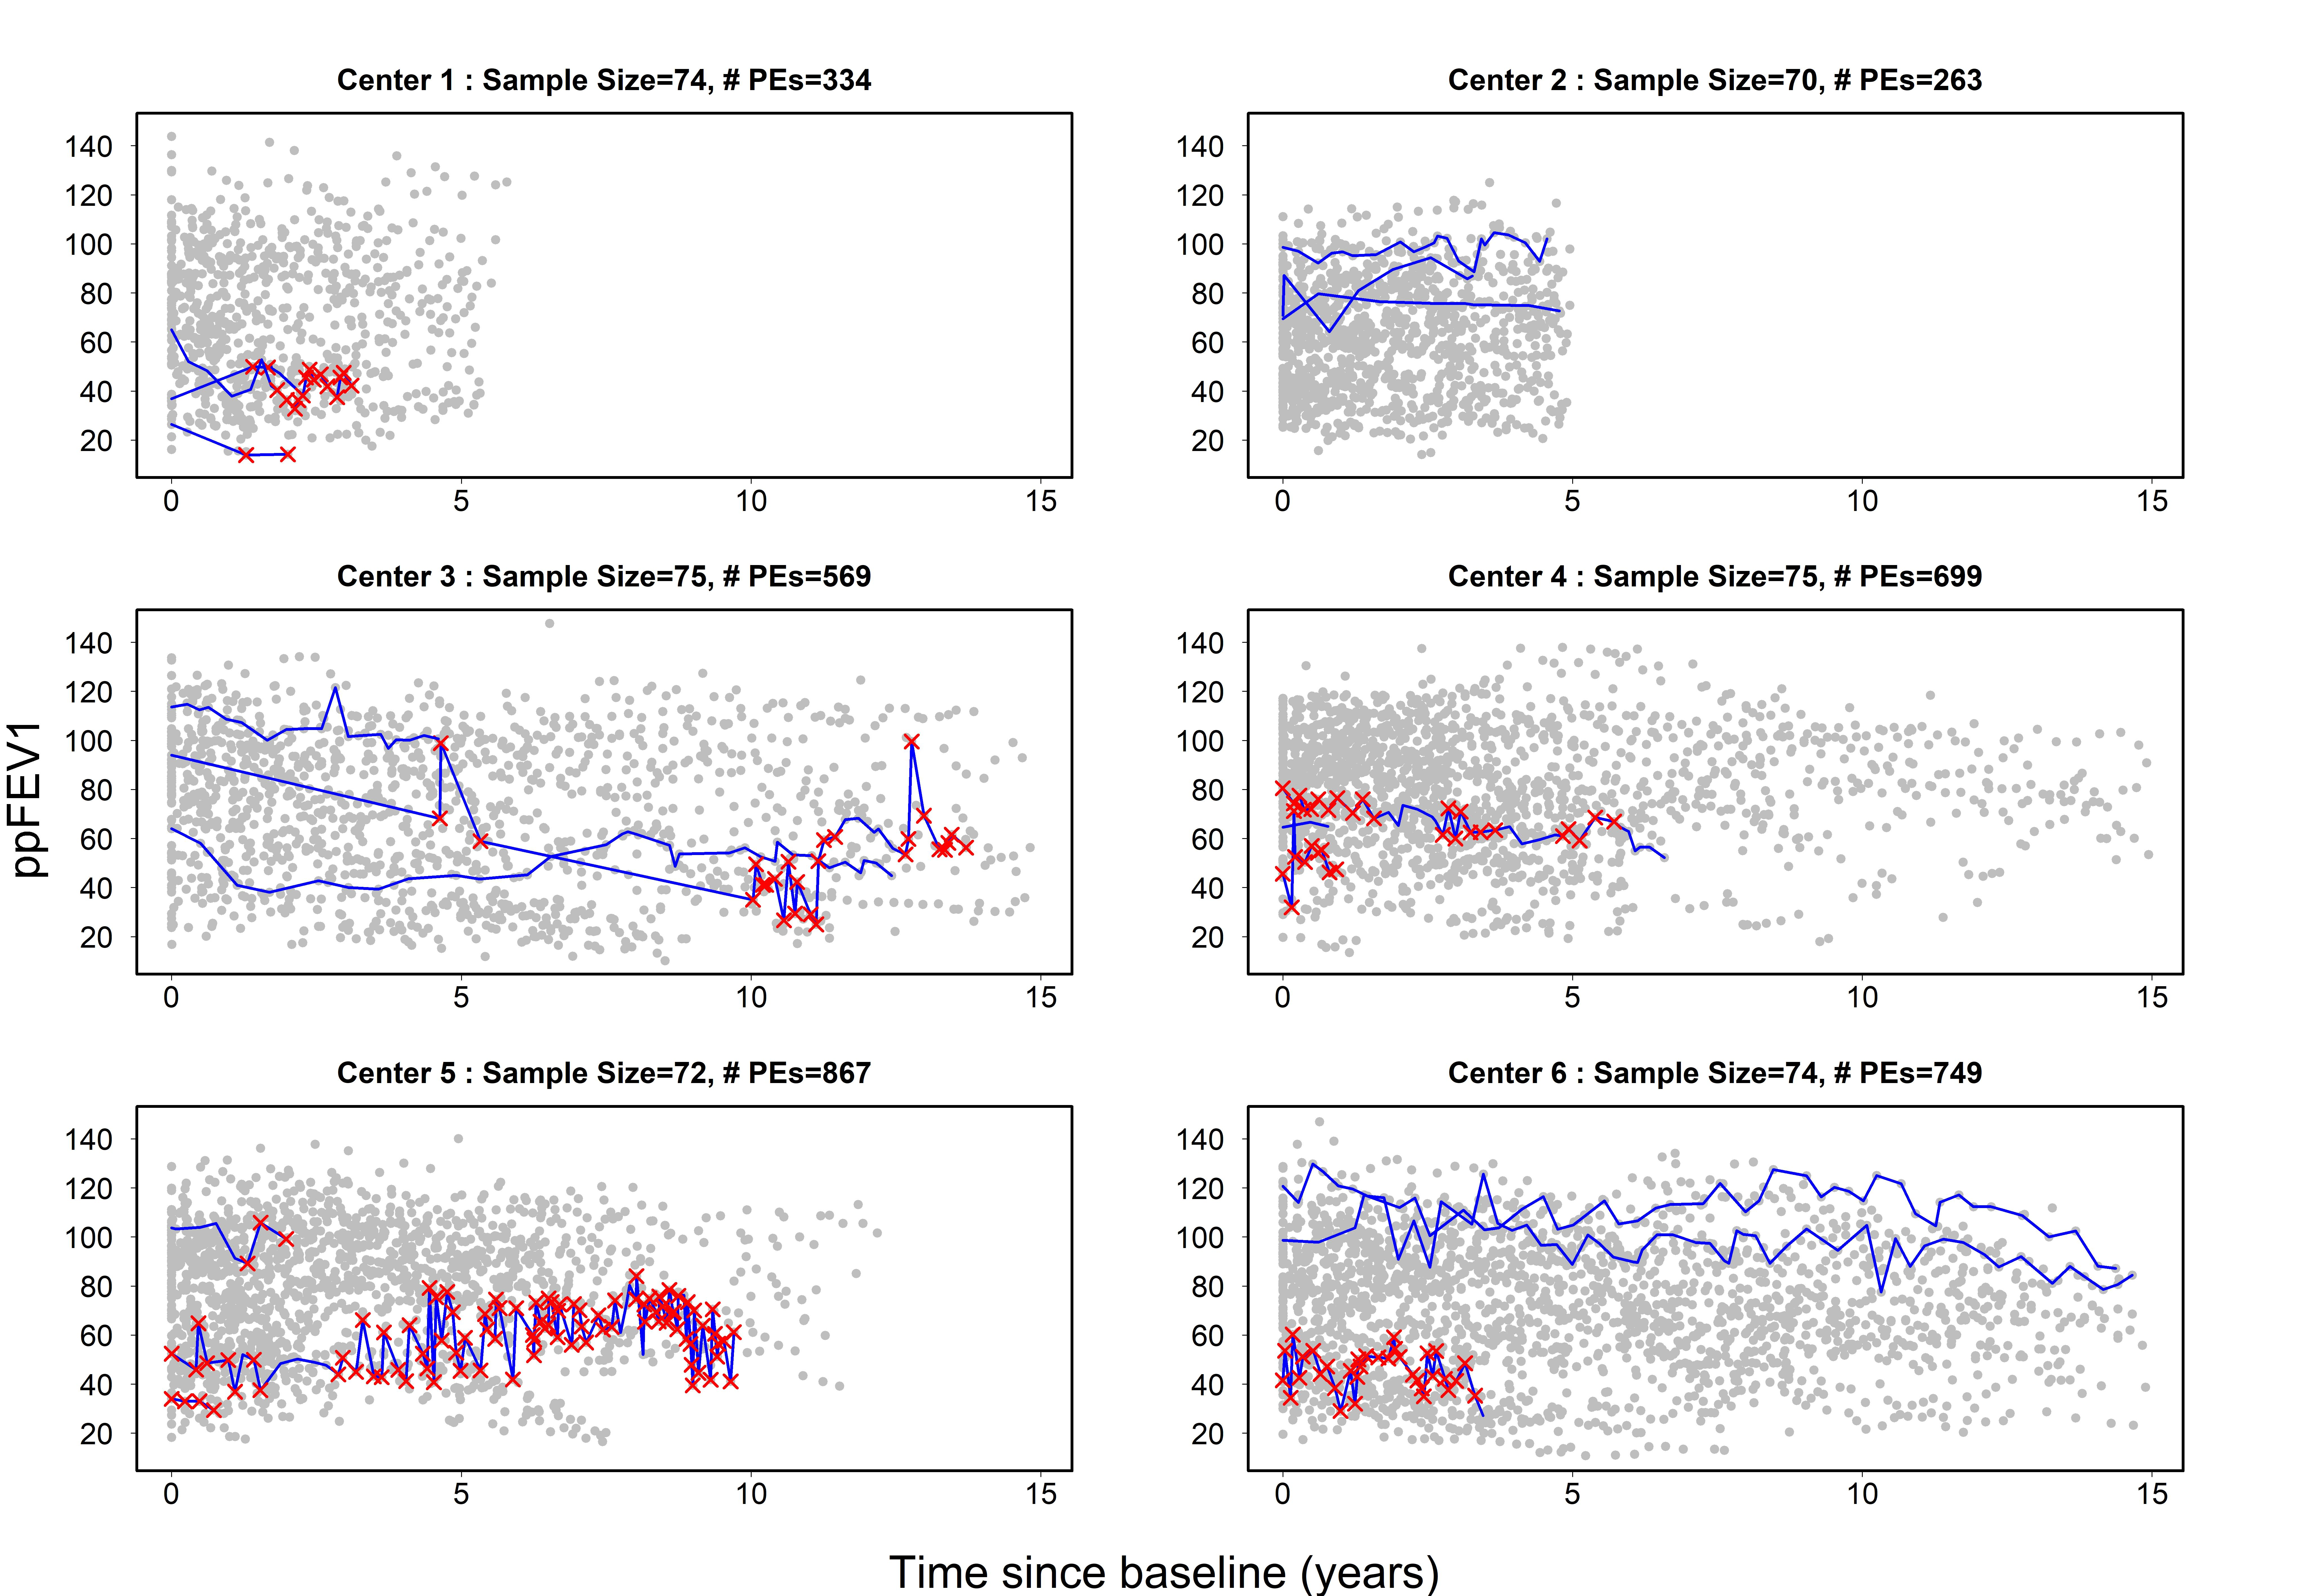
\includegraphics[width=\textwidth]{Figures/Chp3_trajectory.jpg}
\caption{Observed ppFEV1 against time since baseline (in years) for each center. Within each plot: three random specific profiles (solid blue line), observed values (gray dot) and recurrent PE events (red cross)}
\label{fig:chp3_traj}
\end{figure}

\subsection{Model Estimation}

For the sake of internal validation, we split our data into training and masking cohorts without loss of patients. For patients never experience PE event, we mask last period of their observations in terms of quantiles, while for rest of patients, we mask their last observed PE event. Analogously to the Chapter \ref{chp2}, we select predictors from aforementioned variables by \emph{Stepwise} method by a two-stage approach. To the end, we consider the following risk factors: i) For longitudinal submodel: baseline ppFEV1, time, quadratic of time, number of PEs within prior year, birth cohort, infection with pa and gender; ii) For event submodel: number of previous PEs, insurance use at baseline and gender. We examine a total of eight models (four joint models plus four two-stage models) and their comparisons with respect to LOOIC are represented in Table \ref{tab:chp3_comp}. Undoubtedly, all joint models are superior than corresponding two-stage models. From the statistical sight, the joint model with current value of ppFEV1 as the association structure in a calendar time scale outperforms others with the lowest LOOIC. Nonetheless, the choice between calendar time and gap time also depends on clinical interests and predictive performance. For illustration purpose, we pick the 'optimal' model from statistical perspective and its estimations with 90\% equal-tail credible intervals are summarized in Table \ref{tab:chp3_est} and convergence diagnosis plots are included in Appendix \ref{app:c}. From results of the longitudinal submodel, having higher ppFEV1 at entry corresponds to a higher ppFEV1 against time which reconciles with previous findings (\cite{TaylorRobinson2012}, \cite{Li2017}). The presence of infections with pa corresponds to worsen an average -1.15 (90\% CI [-1.64, -0.66]) units of ppFEV1. Being a male patient in older birth cohort is associated with higher ppFEV1. The variance component estimates indicate substantial heterogeneity within and between patients, in terms of large $\sigma,\sigma_{u0},\sigma_{u1}$. While less variations are found between centers given a frail $\sigma_b$. For the event submodel, we observe that males had 28.11\% ($exp(\gamma_3)-1$) lower risk to encounter PE compared to females. The usage of insurance at entry increased the risk by 33.64\% ($exp(\gamma_2)-1$), though it might not be statistically significant. One more count added to cumulative PE events is associated with a 1.01\% ($exp(\gamma_1)-1$) increase in the risk of current PE. Center-specific association parameters are all negative. Specifically, every one percentage predicted increase in 'true and unobserved' ppFEV1 would decrease 3.92\%, 4.88\%, 3.92\%, 3.92\%, 2.96\%, 3.92\% for the PE risk in Center 1 to Center 6, respectively. The non-zero center-specific Weibull shape parameters and frailty term are believed to facilitate the flexibility of the joint model for multi-center cohorts. 

\begin{table}[H]
  \small\sf\centering
   \captionsetup{justification=centering}
\caption{Model comparisons with the boldface as the smallest LOOIC}
\label{tab:chp3_comp}
 \begin{threeparttable}
\begin{tabular}{l|l|l|l|l}
\toprule
Association + Time scale & Model & $\mbox{LOOIC}$ \tnote{a} (SE\tnote{b} )  & $\mbox{LOOIC}_1$\tnote{c} (SE\tnote{b} ) & $\mbox{LOOIC}_2$\tnote{d} (SE\tnote{b} ) \\ \hline
\multirow{2}{*}{Slope + Gap} & Joint Model &  52551.9 (383.1) &	52490.3                                                 (231.5) &  61.6 (151.6) \\
                             & Two-stage Model & 52578.8 (385.7) &	52460.9 (232.3) & 117.9 (153.4)               \\ \hline
\multirow{2}{*}{Slope + Calendar} & Joint Model & 52563.0 (389.4) & 52473.1 (231.9) & 89.9 (157.5) \\
                                  & Two-stage Model & 52575.5 (390.2) & 52460.9 (232.3) & 114.6 (157.9) \\ \hline
\multirow{2}{*}{Value + Gap} & Joint Model & 52574.8 (383.4) & 52491.1 (230.6) & 83.7 (152.8)\\ 
                             & Two-stage Model & 52602.4 (384.5) & 52460.9 (232.3) & 141.5 (152.2)
                                            \\ \hline
\multirow{2}{*}{\textbf{Value + Calendar}} & \textbf{Joint Model} &                     \textbf{52537.3 (386.2)} &                                                            52486.4 (231.1) & 50.9 (155.1) \\ 
                                 & Two-stage Model & 52551.3 (388.3) &	52460.9 (232.3) & 90.4 (156)\\
\bottomrule
\end{tabular}
 \begin{tablenotes}[para]
    \footnotesize
        \item[a] Joint model; \item[b] Standard error approximated as byproduct of \emph{loo} package; \item[c] Longitudinal submodel; \item[d] Event submodel
    \end{tablenotes}
 \end{threeparttable}
\end{table}

\begin{table}[H]
  \small\sf\centering
  \captionsetup{justification=centering}
   \caption{Model estimations under Joint Model: Value+Calendar} \label{tab:chp3_est}
    \begin{threeparttable}
  \begin{tabular}{lcccccccc}
    \toprule
  & mean \tnote{1} & sd \tnote{2} & q5 \tnote{3} & q95 \tnote{3} & rhat \tnote{4} & ess\_bulk \tnote{5} & ess\_tail \tnote{6}\\
 \midrule
  \rowcolor{Gainsboro!60}
   \bf Longitudinal submodel &&&&&&& \\
    $\beta_0$ (intercept at age 6 years) & 7.59 & 1.59 & 5.09 &	10.15 &	1.00 & 713.45 & 1017.42 \\
    $\beta_1$ (baseline ppFEV1) & 0.86 & 0.02 &	0.83 & 0.89 & 1.00 &	553.14 & 1026.96\\
    $\beta_2$ (time since baseline) & -1.12	& 0.22 & -1.48 & -0.76 & 1.00 & 507.77 & 850.71\\
    $\beta_3$ ($\mbox{time since baseline}^2$) & -0.11 & 0.02 &	-0.14 &	-0.09 & 1.00 & 1049.14 & 1517.04\\
    $\beta_4$ (number of PEs within prior year) & -0.33 & 0.05 &	-0.4 & -0.25 & 1.00 & 1742.33 & 1373.07\\
    $\beta_5$ (birth cohort\tnote{$\ast$} $[1988, 1993)$) &3.17 &	1.15 & 1.28 & 5 & 1.00 &	592.67 & 961.08\\
    $\beta_6$ (birth cohort $[1993, 1998)$) & 3.48 & 1.22 &	1.32 & 5.46 & 1.00 & 503.65 &	885.29 \\
    $\beta_7$ (birth cohort $>$1998) & 4.57 & 1.24 & 2.49 &	6.69 & 1.00 &	474.94 & 805.76\\
    $\beta_8$ (pa) & -1.15 & 0.3 & -1.64 & -0.66 & 1.00 & 3771.81 &	1534.25\\
    $\beta_9$ (gender\tnote{$\ast$}  male)  & 1.59 &	0.83 & 0.23 & 2.93 & 1.01 &	470.46 & 924.86\\
    $\sigma$ (measurement error)& 9.07 & 0.08 & 8.94 & 9.2 & 1.00 & 2531.6 & 1556.46\\
    $\sigma_b$ (between centers, intercept) & 1.65 &	1.02 & 0.37 & 3.59 & 1.00 & 396.71 & 382.91\\
    $\sigma_{u0}$ (between patients, intercept) & 6.78 & 0.31 & 6.27 & 7.29 &	1.00 & 784.14 &	1288.57\\
    $\sigma_{u1}$ (between patients, slope)& 3.02 & 0.18 & 2.73 & 3.33 &	1.01 & 340 & 797.25\\
    $\rho$ (correlation, intercept and slope) & 0.18 &	0.07 & 0.06 & 0.3 &	1.01 & 193.5 & 482.79\\
     \rowcolor{Gainsboro!60}
  \bf Event submodel &&&&&&& \\
    $\gamma_0$ (intercept at age 6 years) & 2.02 & 0.28 & 1.57 & 2.5 & 1.00 &	246.96 & 484.67\\
    $\gamma_1$ (number of previous PEs) & 0.01 &	0 &	0 &	0.02 & 1.00 &	1991.24 & 1683.3\\
    $\gamma_2$ (baseline insurance use) & 0.29 & 0.19 &	-0.02 &	0.6 &	1.00 & 307.03 &	651.51\\
    $\gamma_3$ (gender\tnote{$\ast$}  male) & -0.33 & 0.19 & -0.64 & -0.02 & 1.00 &	265.64 & 564.24\\
    $\delta_1$(weibull shape, Center 1)  & 1.24 & 0.09 &	1.1 & 1.38 & 1.00 &	1975.36 & 1535.57\\
    $\delta_2$(weibull shape, Center 2)  & 1.01 & 0.08 &	0.88 & 1.13 & 1.00 & 2476.21 & 1642.13\\
    $\delta_3$(weibull shape, Center 3)  &1.28 &	0.07 & 1.16 & 1.4 &	1.00 & 754.97 &	1167.62\\
    $\delta_4$(weibull shape, Center 4)  & 1.26 & 0.06 &	1.16 & 1.36 & 1.00 & 1780.2 & 1785.08\\
    $\delta_5$(weibull shape, Center 5)  & 1.24 & 0.06 &	1.15 & 1.34 & 1.00 & 1466.17 & 1421.63\\
    $\delta_6$(weibull shape, Center 6)  & 1.07 & 0.05 &	0.98 & 1.15 & 1.00 & 1152.13 & 929.47\\
    $\sigma_v$(between patients, frailty)  & 1.6 &	0.1 & 1.44 & 1.77 &	1.00 & 527.68 &	762.6\\
     \rowcolor{Gainsboro!60}
 \bf Association &&&&&&& \\
    $\alpha_1$ (submodel link, Center 1) & -0.04 & 0 & -0.05 & -0.03 & 1.01 &	455.98 & 786.05\\
    $\alpha_2$ (submodel link, Center 2) & -0.05 & 0.01 &	-0.06 &	-0.04 &	1.00 & 331.54 &	639.72\\
    $\alpha_3$ (submodel link, Center 3) & -0.04 & 0 & -0.05 & -0.04 & 1.00 &	455.63 & 797.91\\
    $\alpha_4$ (submodel link, Center 4) & -0.04 & 0 & -0.04 & -0.03 & 1.01 &	359.67 & 666.75\\
    $\alpha_5$ (submodel link, Center 5) & -0.03 & 0 & -0.03 & -0.02 & 1.01 &	323.03 & 590.15\\
    $\alpha_6$ (submodel link, Center 6) & -0.04 & 0 & -0.05 & -0.04 & 1.01 &	381.33 & 895.84\\
    \bottomrule
  \end{tabular}
 \begin{tablenotes}[para]
    \footnotesize
    \item[1] posterior mean; \item[2] Monte Carlo standard deviation; \item[3] posterior quantiles at 5\% and 95\%; \item[4] potential scale reduction factor (at convergence, rhat=1) \item[5] bulk effective sample size; \item[6] tail effective sample size; \item[$\ast$] Reference: Birth cohort $<1988$; Gender female
    \end{tablenotes}
    \end{threeparttable}
\end {table}

\subsection{Model Diagnostics}

In this section, we validate the assumptions of our joint model (Value+Calendar) through basic residual tools by following the methodology addressed in \cite{Rizopoulos2012d}. For the longitudinal submodel, we implement conditional standardized residuals to check the assumptions of homoscedasticity and normality (see Plot A in Figure \ref{fig:chp3_diag}). We observe that there is no systematic trend from the fitted loess curve, despite some heavy-tailed issues (see Plot B in Figure \ref{fig:chp3_diag}). For the event submodel, we investigate the martingale residuals based on the counting process. Subject-specific martingale residual at time $t$ can be viewed as the difference between the observed number of events by $t$, and the expected number of events by the same time. The fitted zero loess curve illustrates the reasonable performance of the event submodel, despite some outliers. Another diagnostic method, which is called Cox-Snell residuals (\cite{Cox1968}), can be utilized to compare the observed distribution of cumulative hazard with the expected one unit exponential distribution. Cox-Snell residuals are reserved for the time-to-event case, hence we estimate the subject-specific cumulative hazard for the first PE event. Kaplan-Meier estimate (\cite{Kaplan1958}) of the survival function of the censored Cox-Snell residuals is illustrated in Plot D in Figure \ref{fig:chp3_diag}. We observe acceptable discrepancies between the fit of Kaplan-Meier estimate and the expected asymptotic distribution. Apart from previous Gauss-Kronrod approach, here we evaluate the numerical integrand via \emph{integrate} function of R package \emph{stats} (v4.0.2, \cite{R2020}).     

\begin{figure}[H]
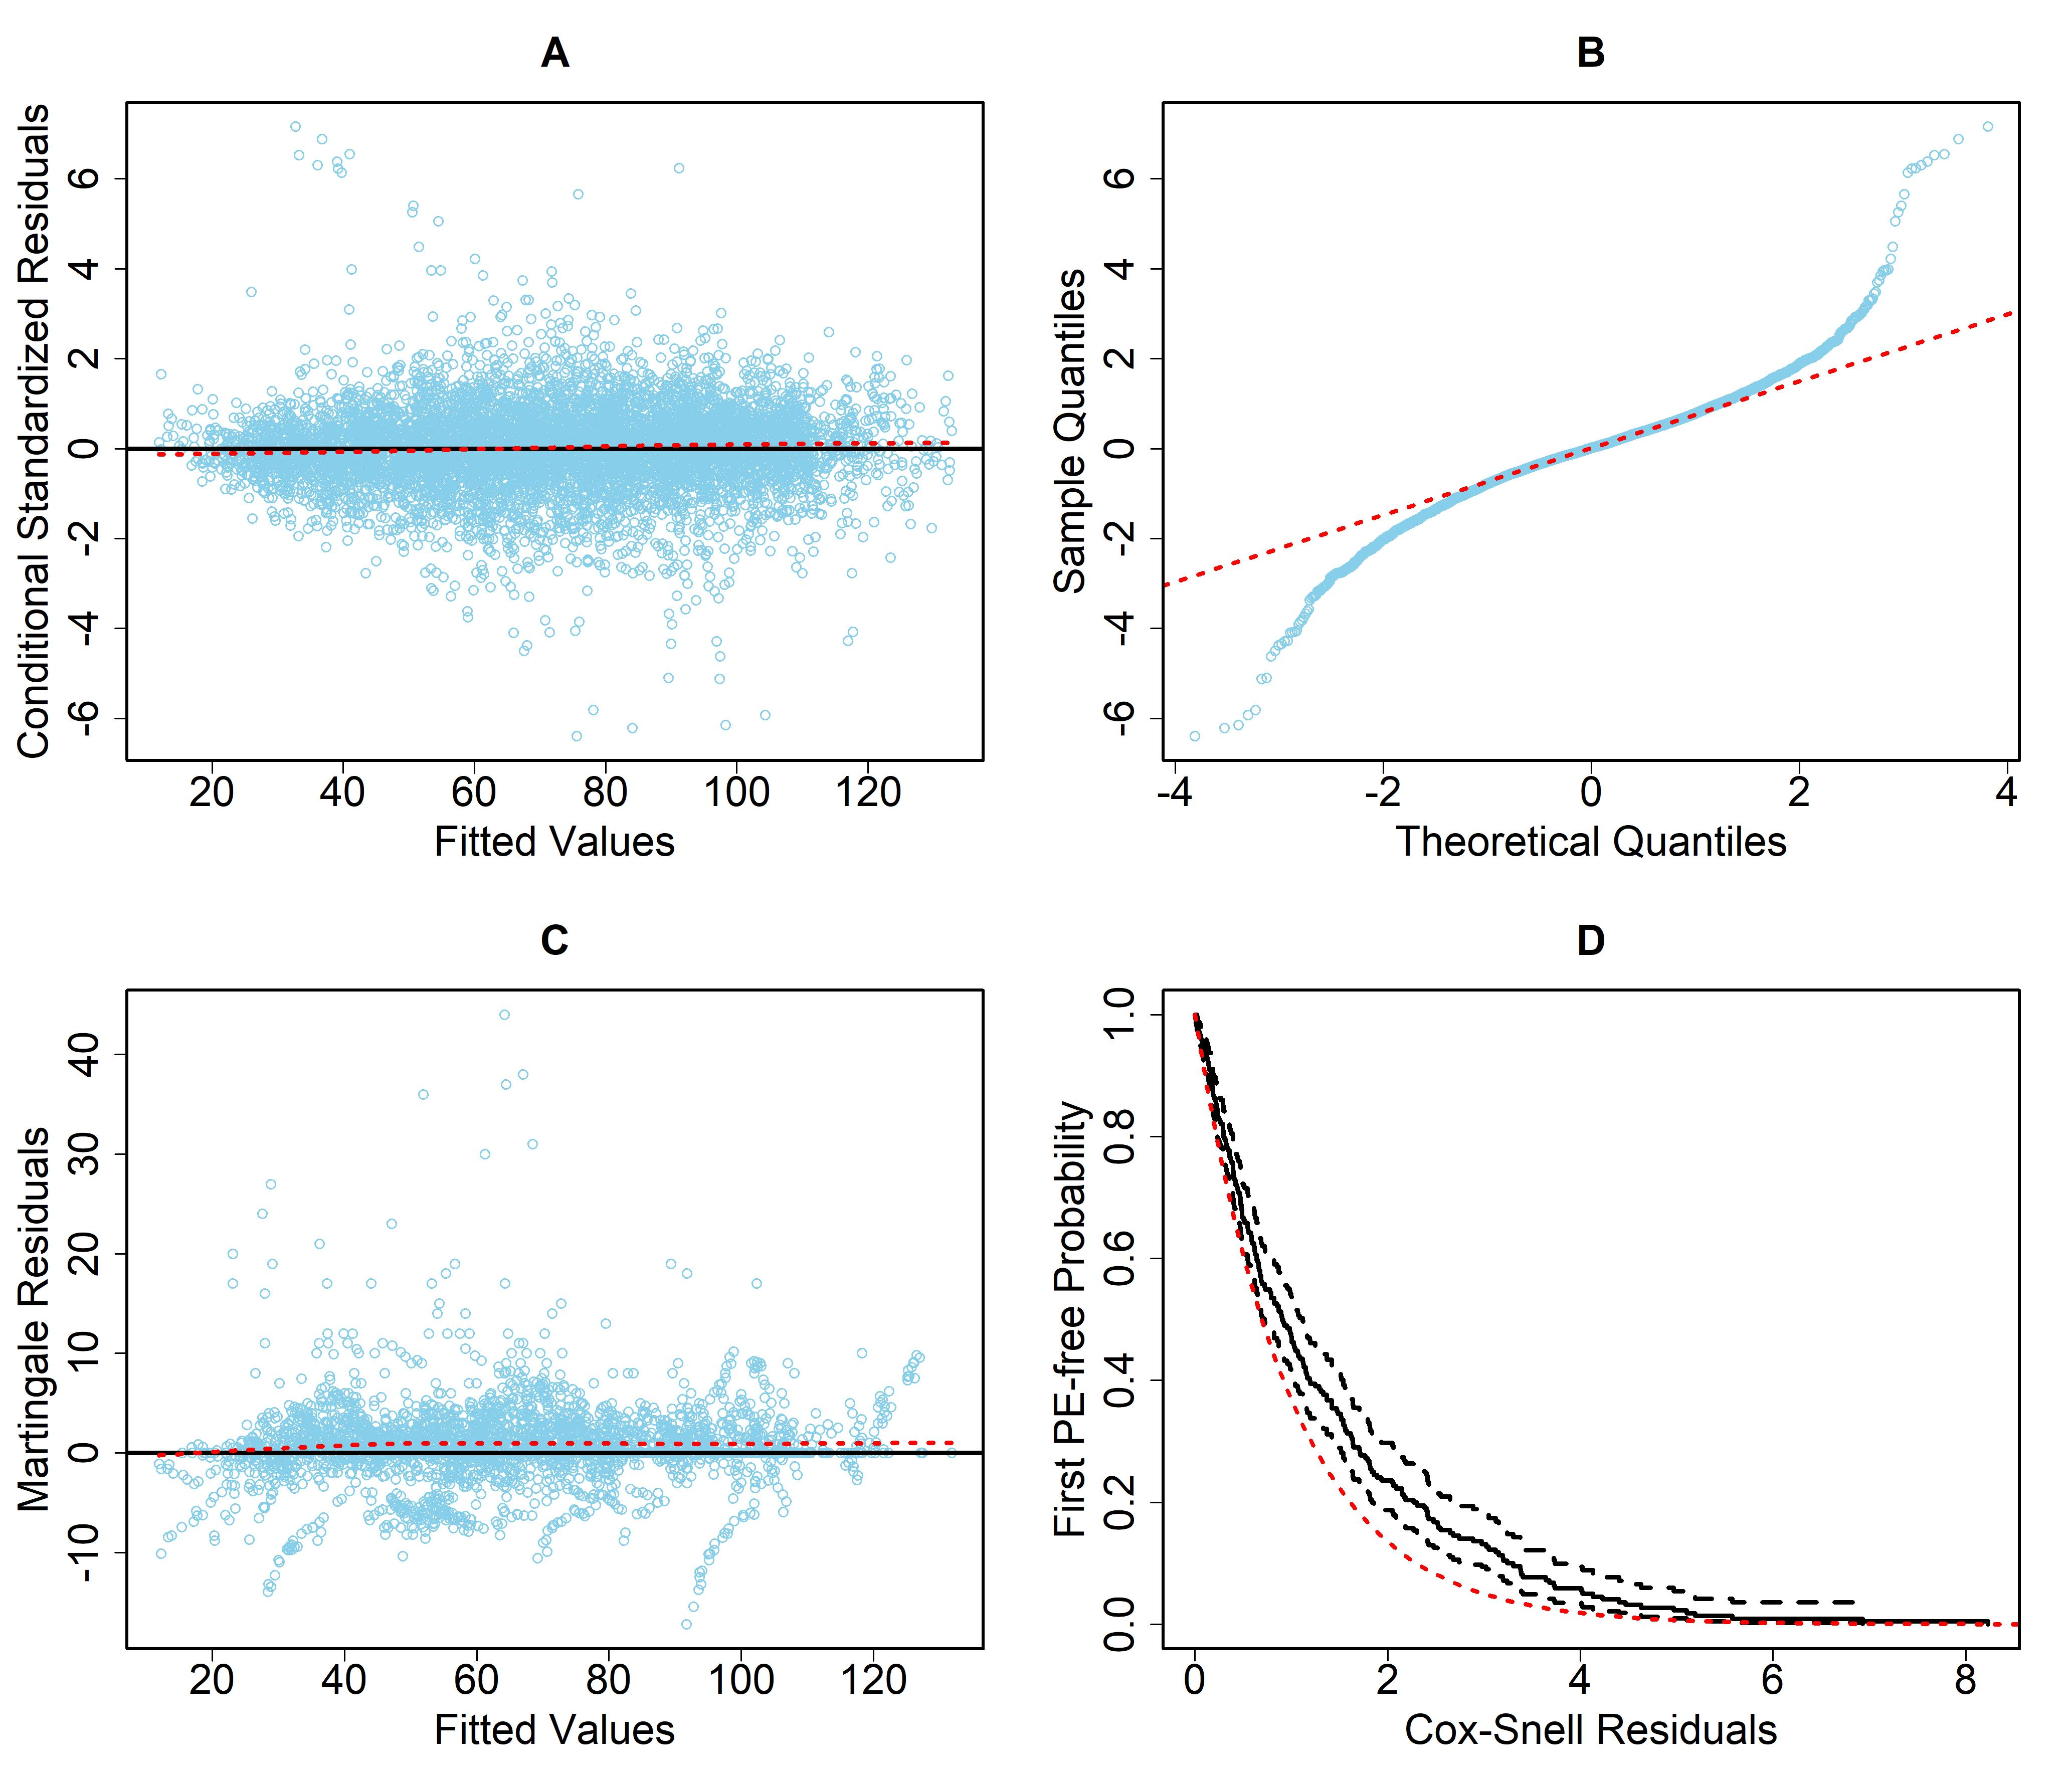
\includegraphics[width=0.9\textwidth]{Figures/Chp3_DIAG.jpg}
\caption{Residuals diagnostic plot for the proposed joint model. Upper panel: subject-specific standardized residuals versus fitted values (A) and normal Q-Q plot for longitudinal submodel (B). Lower panel: subject-specific martingale residuals versus fitted values (C) and Cox-Snell residuals for event submodel (D). Red dashed lines in A \& C are fitted loess curve; that in B \& D are normal curve and exponential curve, respectively}
\label{fig:chp3_diag}
\end{figure}

\subsection{Predictive Performance}

To assess predictive performance of proposed joint models, we compute time-dependent AUC and MPE for each joint model under various future time scenarios and results are shown in Table \ref{tab:myauc}. Unlike the conventional method used in \cite{Ren2021}, that is to assign a common prediction start time ($t$), we characterize individual prediction time ($t_{li}$) from the end time of each patient's last available encounter. The future times ($t'$) are summarized by the quartile of their stop times and the concept of patients at risk denotes that patients have not yet experienced the next occurrence of PE at $t'$.  

All joint models represent the excellent discriminate and calibrate capability in the longer term run. Figure \ref{fig:chp3_pred} forecast random patients who are still at risk after their last observed measurements under the joint model Value+Calendar. We note that Patient 202 and Patient 284 represent two extreme cases, suggesting that higher lung function reduces the risk of the next PE event, while the latter patient needs a timely care and prevention given high risk for the next PE event. From virtual inspection, we observe that averaged ppFEV1 value and frequency of previous PE occurrences are not ignorable risk factors for the prognostic probability of the next PE event.

\begin{table}[H]
  \small\sf\centering
  \captionsetup{justification=centering}
\caption{Predictive performance of proposed joint models}
\label{tab:myauc}
\begin{threeparttable}
\begin{tabular}{c|c|l|c|c}
\toprule
\textbf{Future time (years)} & \textbf{Num Patients at risk} & \textbf{Joint Model} & \textbf{AUC} & \textbf{MPE} \\ \hline
\multirow{4}{*}{2.73} & \multirow{4}{*}{118} & Slope + Gap & 0.61 &	0.28 \\
                      &                      & Slope + Calendar & 0.64 & 0.27 \\
                      &                      & Value + Gap & 0.66 & 0.27 \\
                      &                      & Value + Calendar & 0.68 & 0.26 \\ \cline{1-5}
\multirow{4}{*}{5.10} & \multirow{4}{*}{141} & Slope + Gap &	0.89 & 0.14 \\
                     &                      & Slope + Calendar & 0.88 & 0.14 \\
                     &                      & Value + Gap & 0.90 & 0.14 \\
                     &                      & Value + Calendar & 0.88 &	0.14\\ \cline{1-5}
\multirow{4}{*}{7.84} & \multirow{4}{*}{107} & Slope + Gap & 0.92 &	0.12 \\
                      &                      & Slope + Calendar & 0.91 & 0.13 \\
                      &                      & Value + Gap & 0.92 &	0.12 \\
                      &                      & Value + Calendar & 0.92 & 0.13\\ 
\bottomrule
\end{tabular}
\begin{tablenotes}[para]
\footnotesize
Abbreviation: AUC=area under curve; MPE=mean predictive error
\end{tablenotes}
\end{threeparttable}
\end{table}

\begin{figure}[ht]
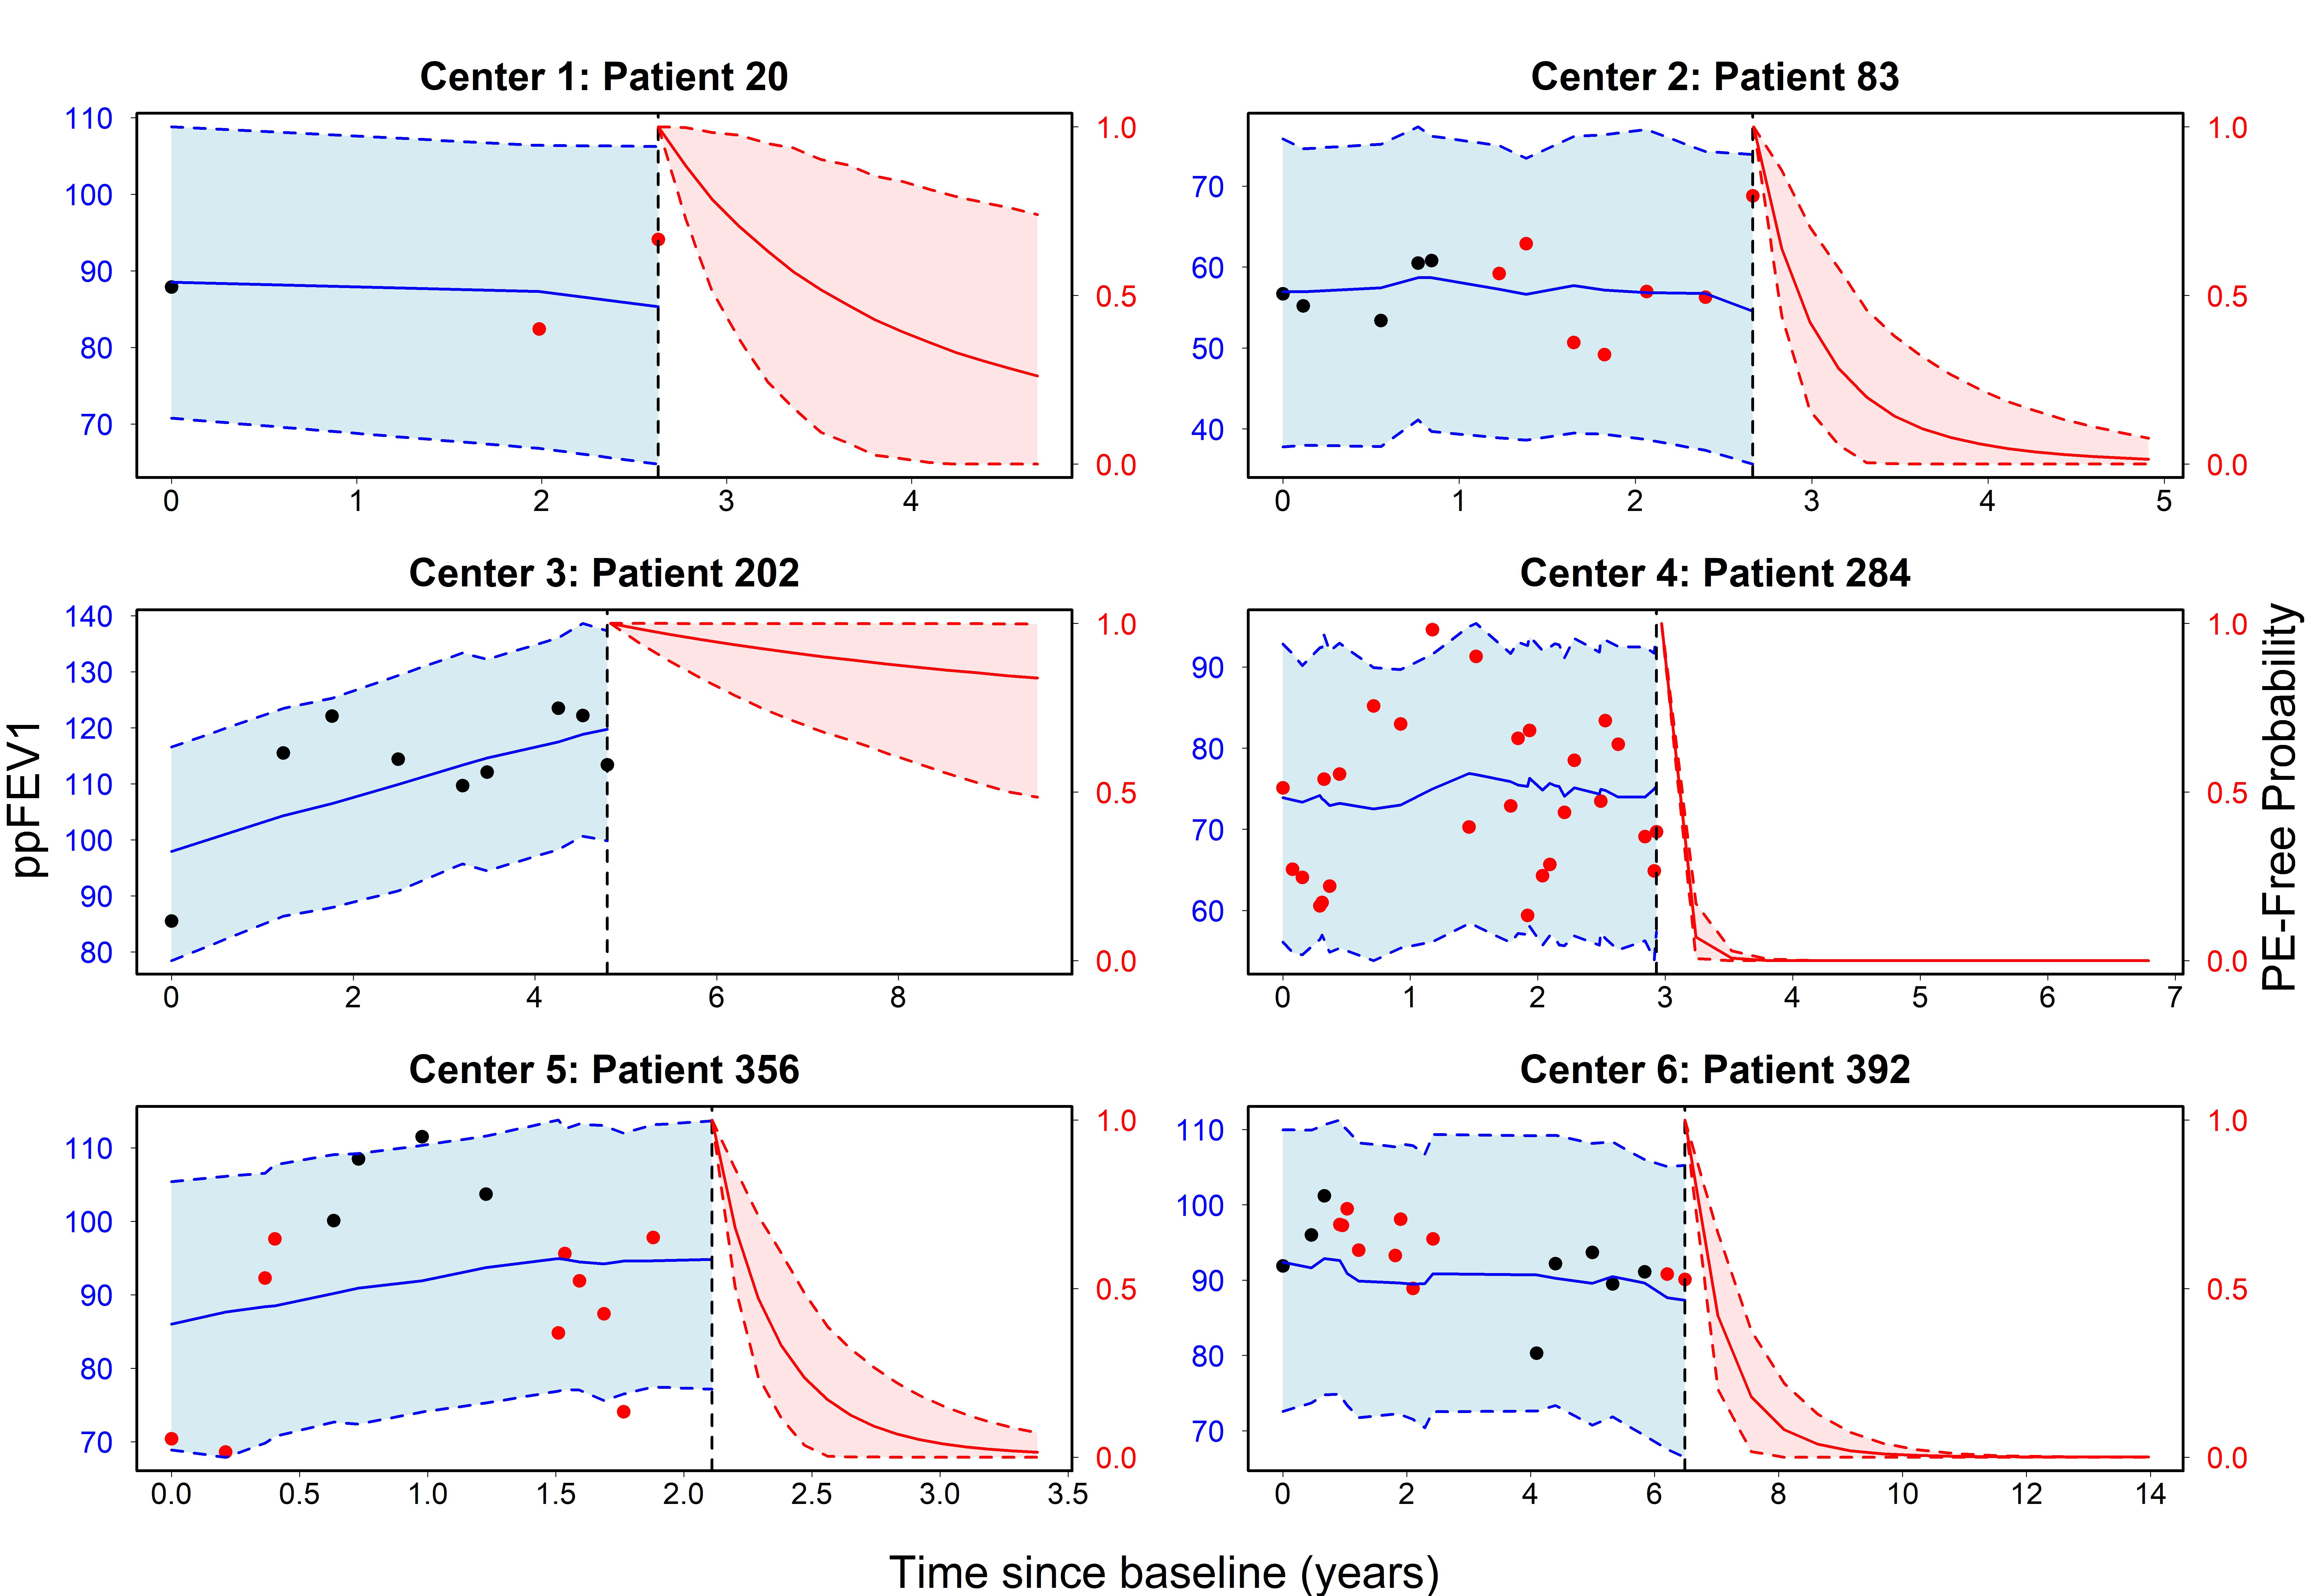
\includegraphics[width=\textwidth]{Figures/Chp3_PRED_PLOT2.jpg}
\caption{Individual predictions against time by centers, including observed ppFEV1 (dots) illustrated by PE event (red dots) and non-PE event (black dots), fitted value of ppFEV1 (blue lines), prognostic PE-free probability (red lines) and 95\% credible intervals (bands)}
\label{fig:chp3_pred}
\end{figure}

\section{Discussion} \label{sec:chp3_diss}

In this chapter, we have proposed a multilevel Bayesian joint model for a monitoring CF data depicted by hierarchical structures and irregularly clinical visits. Our novel model allows for center-specific association parameters to quantify the strength of the correlation between the two processes and such approach facilitate individual prognosis towards personalized medical monitoring. Furthermore, we provide detailed simulation algorithm and \emph{Stan} codes by extending the work of \cite{Brilleman2018}. Despite the large cost of computing time due to large sample size and approximation using Gauss-Kronrod quadrature rule, Bayesian methodology provides convincing benefits, especially lead to posterior predictive distributions and release the numerical integral burden through Monte Carlo samplings.

The availability of robust software packages is limited. In Chapter \ref{chp1}, we have introduced briefly R packages \emph{JMBayes2} and \emph{rstanarm}. There also exists R package frailtypack (\cite{Rondeau2019}), which allows for joint nested frailty models in the context of the joint modeling for recurrent events with terminal event, for hierarchically clustered data. Notwithstanding that it closely relates to our topic, it adapts maximum penalized likelihood estimation rather than the Bayesian approach. For this sake, we implement our own R code with \emph{Stan} programs via \emph{CmdStanR} interface to Stan (\cite{Gabry2022}). To enhance rigor and reproducibility of our proposed model, the example codes have been posted in Appendix \ref{app:c}.  

This article would be considered in the light of some limitations and interesting extensions. We limit our work on recurrent events without presence of terminal event. However, it may be necessary to include additional submodel for a terminal event in the context of an extended joint model in the future research. Notwithstanding we present the individual prognostic rationale for in-sample patients, there exists great practical and theoretical interest to investigate out-of-sample predictions in terms of dynamic feature, which was proposed with novelty for univariate joint model in \cite{Proust-Lima2009} and \cite{Rizopoulos2011}; applied for joint model with recurrent events in \cite{Ren2021} or joint model for recurrent events with a terminal event in \cite{Mauguen2013}. Furthermore, with respect to the specific forecast period, it might be interesting to access the predictive performance at several clinical relevant window widths (e.g., age 18 to 23 or age 25 to 30), which are dependent on frequencies of (next) PE events. Though predictive probability of next event is welcome, an alternative measure is mean residual life (MRL), which provides the expected time to the next event occurrence (\cite{Deep2020}). The advantage of MRL lies in its clinical interpretation between physicians and patients. We utilize ubiquitous random intercept-slope model for the longitudinal submodel, while it can be replaced by some other novel Gaussian process models, nevertheless, the complexity is unlikely to be warranted. In this paper, we barely include time-varying covariates for the event submodel, hence, more time-dependent risk factors could be further investigated. With respect to various baseline hazard function candidates, alternatives such as bsplines, piecewise-constant are undergoing. Lastly, we investigate the routine diagnostics of joint model, which has not received much attention in the joint modeling literature. Readers who are interested in a thorough discussion about this topic can refer to \cite{Rizopoulos2012d} for some new insights. 

